\documentclass[12pt]{article}
\usepackage[T2A]{fontenc}
\usepackage[utf8]{inputenc}
\usepackage[english, russian]{babel}

\usepackage{graphicx}
\graphicspath{ {./images/} }

\usepackage{wrapfig}
\usepackage[rightcaption]{sidecap}

\begin{document}
\title{Электрический импульс центрально-симметричного взрыва плазмы}
\author{А.Ю. Дроздов}
\date{Май - декабрь 2020}

\begin{titlepage}
\maketitle
\end{titlepage}


\begin{abstract}
В данной работе представлены результаты моделирования центрально симметричного взрыва с использованием запаздывающих потенциалов Лиенара Вихерта и скалярно-векторного потенциала Менде. Показана непригодность потенциала ЛВ для объяснения наблюдаемой в опыте отрицательной полярности импульса и непригодность скалярно-векторного потенциала Менде для объяснения величины измеренного импульса.
\end{abstract}



\section{Введение}

Одной из нерешённых проблем современной электродинамики является проблема электромагнитного импульса ядерного взрыва. В журнале Инженерная физика появилась статья \cite{Mende2013} в которой была сделана попытка объяснить это явление в рамках концепции скалярно-векторного потенциала. Эта концепция по мнению ее автора предполагает зависимость скалярного потенциала заряда от скорости.

Такая зависимость была получена из анализа законов индукции электрического поля магнитным и магнитного поля электрическим, записанных с использованием субстанциональной производной полевых функций в форме, инвариантной относительно преобразований координат классической физики, включающих преобразования Галилея.

Приводятся также экспериментальные данные, которые заключаются в появлении электрического потенциала на сверхпроводящих обмотках и торах при введении в них постоянного тока \cite{Edwards1976} \cite{Roser1962} \cite{Baker1964} \cite{Mende1993}.

В 2015 году появилась публикация \cite{Mende2015} с описанием модельного эксперимента моделирующего возникновение ЭМИ посредством регистрации импульса возникающего при электрическом взрыве медной проволочки. Анализу результатов данного модельного эксперимента и посвящена данная работа.

Для начала следует отметить, что попытка объяснить электромагнитный импульс центрально симметричного взрыва плазмы в рамках концепции скалярно-векторного потенциала является ошибочной. Чтобы в этом убедиться достаточно привести рассуждения Ф.Ф. Менде, применённые при выводе скалярно-векторного потенциала, но для случая случае центрально-симметричного движения зарядов.
Действительно, пусть мы имеем три ИСО: первая неподвижная, вторая движется со скоростью $dv$, а третья со скоростью $2dv$. В третьей ИСО расположен заряженный стержень. Во второй появляется прибавка магнитного поля $dB$. А в первой прибавка электрического поля $dE$.
Однако в случае разогретой плазмы мы имеем не единственный движущийся заряженный стержень. Таких "стержней", движущихся во всех направлениях с различными скоростями очень много.

В случае разогретой плазмы, имеющей сферическую симметрию, о распределении "стержней" по скоростям можно утверждать следующее: сколько стержней движется со скоростью $2dv$, столько же движется со скоростью $-2dv$.

Таким образом для разбора ситуации нам достаточно ввести в рассмотрение ещё две ИСО: четвёртая, движущаяся со скоростью $-dv$. И пятая, движущаяся со скоростью $-2dv$. При этом в пятой ИСО имеется ещё один заряженный стержень.

В четвёртой ИСО появляется прибавка магнитного поля $-dB$. А в первой ИСО появляется прибавка электрического поля$-dE$.
Таким образом мы видим, что согласно предложенного Менде при выводе скалярно-векторного потенциала механизма в конфигурации сферически симметричной разогретой плазмы суммарная прибавка электрического поля равна нулю.

Причина такого вывода заключается в том, концепция скалярно-векторного потенциала Менде основана на «перпендикулярном» механизме образования прибавки электрического поля. И поэтому его применение может быть распространено на токовые системы обычного типа, в которых движущиеся электроны имеют преимущественное направления движения в какую-либо сторону, например, упомянутые выше сверхпроводящие обмотки и торы. Но эта концепция не применима к сферически симметрическому электрическому вибратору.

Кроме того нужно иметь ввиду, что при выводе формулы скалярно-векторного потенциала Менде была допущена принципиальная ошибка, заключающаяся в том, что формула, полученная для потенциала движущегося заряженного длинного стержня не может быть преобразована в формулу потенциала движущегося точечного заряда одним лишь увеличением степени  $r$  в знаменателе. При детальном повторении рассуждений Менде, но не с движущимся заряженным стержнем, а с движущимся точечным зарядом возникает необходимость учёта того обстоятельства, что угол между вектором скорости движущегося заряда и радиус вектором от заряда к точке наблюдения может отличаться от 90 градусов. При учете этого обстоятельства получается, что формула для скалярно-векторного потенциала движущегося точечного заряда неверна.

\section{Двойной электрический слой на сфере}

Рассмотрим скалярный потенциал сферически заряженного конденсатора, у которого внутренняя поверхность заряжена положительно, а внешняя отрицательно
	\[\varphi =\int\limits_{{{S}^{+}}}{\frac{{{\sigma }^{+}}}{{{R}^{+}}}dS+}\int\limits_{{{S}^{-}}}{\frac{{{\sigma }^{-}}}{{{R}^{-}}}dS}\] 	
где ${{R}^{+}}$и ${{R}^{-}}$ расстояния от точек на поверхности заряженных сфер к точке наблюдения.

Радиус вектор от частиц слоя к точке наблюдения расположенной на оси $z$ на расстоянии ${{R}_{0}}$ от центра сферы $\overrightarrow{R}=-x\widehat{i}-y\widehat{j}+\left( {{R}_{0}}-z \right)\widehat{k}$, где $x=r\cdot \sin \theta \cdot \cos \varphi $ , $y=r\cdot \sin \theta \cdot \sin \varphi $ и \[z=r\cdot \cos \theta \] - координаты заряда на поверхности сферы радиуса $r$. Для квадрата радиус вектора можно записать $\overrightarrow{R}\cdot \overrightarrow{R}={{\left( -x \right)}^{2}}+{{\left( -y \right)}^{2}}+{{\left( {{R}_{0}}-z \right)}^{2}}={{x}^{2}}+{{y}^{2}}+{{R}_{0}}^{2}-2{{R}_{0}}z+{{z}^{2}}={{R}_{0}}^{2}-2{{R}_{0}}z+{{r}^{2}}$, откуда расстояние от заряда к точке наблюдения $R=\sqrt{{{R}_{0}}^{2}-2{{R}_{0}}r\cos \theta +{{r}^{2}}}$.

С учетом закона сохранения электрического заряда заряд внутренней обкладки равен заряду внешней $q=4\pi {{r}^{{{+}^{2}}}}{{\sigma }^{+}}=4\pi {{r}^{{{-}^{2}}}}{{\sigma }^{-}}$ таким образом выражение для потенциала обкладки в сферической системе координат с учётом $dS={{r}^{2}}\sin \theta d\varphi d\theta $  можно записать как
	\[\varphi =\int\limits_{\theta =0}^{\pi }{\int\limits_{\varphi =0}^{2\pi }{\frac{\sigma dS}{R}}} = \]
 \[\int\limits_{\theta =0}^{\pi }{\int\limits_{\varphi =0}^{2\pi }{\frac{\frac{q}{4\pi {{r}^{2}}}{{r}^{2}}\sin \theta d\varphi d\theta }{\sqrt{{{R}_{0}}^{2}-2{{R}_{0}}r\cos \theta +{{r}^{2}}}}}} = \]

 \[\frac{q}{4\pi }\int\limits_{\theta =0}^{\pi }{\int\limits_{\varphi =0}^{2\pi }{\frac{\sin \theta d\varphi d\theta }{\sqrt{{{R}_{0}}^{2}-2{{R}_{0}}r\cos \theta +{{r}^{2}}}}}}\]

Где ${R}_{0}$ расстояние от центра сферы к точке наблюдения, расположенной на оси $z$. Интегрируя по $\varphi$ для выражения скалярного потенциала заряженной сферы получим
	\[\varphi =\frac{1}{4\pi }\int\limits_{\theta =0}^{\pi }{\frac{2\pi q\sin \theta d\varphi d\theta }{\sqrt{{{R}_{0}}^{2}-2{{R}_{0}}r\cos \theta +{{r}^{2}}}}}=\frac{1}{2}\int\limits_{\theta =0}^{\pi }{\frac{q\sin \theta d\varphi d\theta }{\sqrt{{{R}_{0}}^{2}-2{{R}_{0}}r\cos \theta +{{r}^{2}}}}}\] 	

Таким образом скалярный потенциал сферического можно рассчитать по формуле
	\[\varphi =\frac{1}{2}\int\limits_{\theta =0}^{\pi }{\frac{+q\sin \theta d\varphi d\theta }{\sqrt{{{R}_{0}}^{2}-2{{R}_{0}}{{r}_{+}}\cos \theta +{{r}_{+}}^{2}}}}+\frac{1}{2}\int\limits_{\theta =0}^{\pi }{\frac{-q\sin \theta d\varphi d\theta }{\sqrt{{{R}_{0}}^{2}-2{{R}_{0}}{{r}_{-}}\cos \theta +{{r}_{-}}^{2}}}}\]

Подставляя численные значения: радиус наружной отрицательной обкладки ${{r}_{-}}=2$ а радиус внутренней положительной обкладки ${{r}_{+}}=1$, заряды обкладок равны друг другу $q=1$

\begin{wrapfigure}{l}{0.6\textwidth}
    \centering
    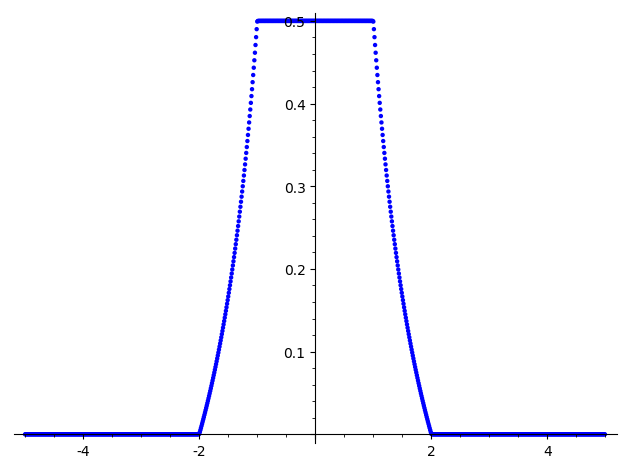
\includegraphics[scale=0.3]{spherical_capascitor_phi_Rneg=2_Rpos=1}
    \caption{Скалярный потенциал сферического конденсатора}
    \label{fig:spherical_capascitor_phi_Rneg=2_Rpos=1}
\end{wrapfigure}

Приходим к классическому выводу, что поле в сферическом конденсаторе не нулевое только между обкладками.

Предположим, что заряженные обкладки двойного электрического слоя движутся в радиальном направлении с различными скоростями ${{v}^{+}}$ и ${{v}^{-}}$. 

Потенциал Лиенара-Вихерта двойного электрического слоя рассчитывается по формуле
	\[\varphi =\int\limits_{{{S}^{+}}}{\frac{{{\sigma }^{+}}}{{{R}^{+}}-\frac{\overrightarrow{{{v}^{+}}}\cdot \overrightarrow{{{R}^{+}}}}{c}}dS+}\int\limits_{{{S}^{-}}}{\frac{{{\sigma }^{-}}}{{{R}^{-}}-\frac{\overrightarrow{{{v}^{-}}}\cdot \overrightarrow{{{R}^{-}}}}{c}}dS}\] 	

Для нахождения скалярного произведения радиального вектора скорости заряда движущегося на поверхности сферы на вектор от заряда в точку наблюдения произведём следующие вспомогательные выкладки

Радиальная скорость частиц слоя радиуса $r$ равна $\overrightarrow{v}=\frac{\overrightarrow{r}}{r}v$ где \[\overrightarrow{r}=x\widehat{i}+y\widehat{j}+z\widehat{k}\] и ${{r}^{2}}={{x}^{2}}+{{y}^{2}}+{{z}^{2}}$ 

Запишем скалярное произведение вектора радиальной скорости частиц на радиус вектор в точку наблюдения
$$\overrightarrow{v}\cdot \overrightarrow{R}=\frac{v}{r}\overrightarrow{r}\cdot \overrightarrow{R}=\frac{v}{r}\left( -x\cdot x-y\cdot y+\left( {{R}_{0}}-z \right)\cdot z \right)=\frac{v}{r}\left( -{{x}^{2}}-{{y}^{2}}-{{z}^{2}}+{{R}_{0}}z \right)$$

$$\overrightarrow{v}\cdot \overrightarrow{R}=\frac{v}{r}\left( -{{r}^{2}}+{{R}_{0}}z \right)$$

подставляя выражение для в сферической системе координат
	$$\overrightarrow{v}\cdot \overrightarrow{R}=v\left( {{R}_{0}}\cos \theta -r \right)$$

Итак, потенциал Лиенара Вихерта заряженной сферы, частицы поверхности которой имеют радиальную скорость $v$ 
	\[\varphi =\frac{q}{4\pi }\int\limits_{\theta =0}^{\pi }{\int\limits_{\varphi =0}^{2\pi }{\frac{\sin \theta d\varphi d\theta }{\sqrt{{{R}_{0}}^{2}-2{{R}_{0}}r\cos \theta +{{r}^{2}}}-\frac{v}{c}\left( {{R}_{0}}\cos \theta -r \right)}}}\] 	

Интегрируя по $\varphi $ 
	\[\varphi =\frac{q}{2}\int\limits_{\theta =0}^{\pi }{\frac{\sin \theta d\theta }{\sqrt{{{R}_{0}}^{2}-2{{R}_{0}}r\cos \theta +{{r}^{2}}}-\frac{v}{c}\left( {{R}_{0}}\cos \theta -r \right)}}\]

В полученных уравнениях координата $r$ и скорость $v$ используется в запаздывающий момент $t'$.
%Рассмотрим сферический конденсатор. Пусть его внутренняя обкладка, заряженная положительно, имеет радиус ${{r}_{+}}=1$ а внешняя отрицательная обкладка имеет радиус ${{r}_{-}}=2$ 


%Расчёт по формуле  скалярного потенциала Лиенара Вихерта (пока что без учёта запаздывания) для двух обкладок сферического конденсатора, в котором внешняя отрицательная обкладка разлетается наружу со скоростью ${{v}_{-}}={}^{1}/{}_{3}c$ , а внутренняя обкладка покоится, имеет вид, показанный на рисунке  \ref{fig:spherical_capascitor_phi_Rneg=2_Rpos=1_vneg=1_3c_without_lagging}

%\begin{SCfigure}[0.9][h]
%   \caption{Скалярный потенциал ЛВ (без запаздывания) сферического конденсатора, внешняя отрицательная обкладка разлетается наружу.}
%   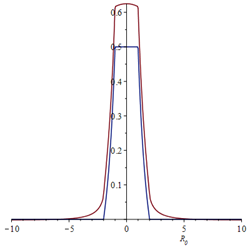
\includegraphics[width=0.4\textwidth]{spherical_capascitor_phi_Rneg=2_Rpos=1_vneg=1_3c_without_lagging}
%   \label{fig:spherical_capascitor_phi_Rneg=2_Rpos=1_vneg=1_3c_without_lagging}
%\end{SCfigure}

%Для сравнения на том же графике показан потенциал конденсатора с покоящимися обкладками

%Скалярный потенциал Лиенара Вихерта (без учёта запаздывания) сферического конденсатора того же размера, в котором внешняя отрицательная обкладка схлопывается внутрь с той же скоростью ${{v}_{-}}=-{}^{1}/{}_{3}c$ . Внутри внутренней положительной сферы появляется потенциальная яма для положительных зарядов.

%Скалярный потенциал Лиенара Вихерта (без учёта запаздывания) сферического конденсатора, в котором обе обкладки - как внешняя, отрицательная, так и внутренняя, положительная, разлетаются наружу. Скорости обкладок ${{v}_{-}}={}^{1}/{}_{3}c$ и${{v}_{+}}={}^{1}/{}_{6}c$. Начальная фаза центрально-симметричного взрыва. 

%Скалярный потенциал Лиенара Вихерта (без учёта запаздывания) сферического конденсатора, в котором положительная обкладка разлетается наружу, а отрицательная обкладка схлопывается внутрь. Обе обкладки движутся навстречу друг другу. Скорости обкладок ${{v}_{-}}=-{}^{2}/{}_{3}c$ и${{v}_{+}}={}^{1}/{}_{3}c$. Потенциальная яма внутри положительной обкладки максимально глубокая. (Ниже будет показано, что учёт запаздывания изменит вид этой потенциальной кривой кардинальным образом).

%Данные расчёты носят чисто иллюстративный характер с целью показать, что для объяснения эффекта появления электрического поля вне сферического конденсатора с движущимися обкладками совершенно не обязательно использовать гипотезу зависимости заряда электрона от скорости его движения.

%Согласно вышеприведенному иллюстративному расчёту по формуле  скалярного потенциала Лиенара-Вихерта без учёта запаздывания, - для начальной фазы центрально симметричного взрыва получается такой эффект, как будто внутри сферического конденсатора, выражаясь языком Менде, «образуется унитарный положительный заряд». Однако в опубликованных результатах своего опыта Менде утверждает, что начальная фаза центрально-симметричного взрыва характеризуется появлением электрического поля такого направления, как будто внутри экспериментальной установки «образуется унитарный отрицательный заряд».

%Для получения более точных результатов потенциала Лиенара Вихерта необходимо, во-первых, учесть явление запаздывания, а во-вторых учесть влияние ускорения зарядов. Кроме того, необходимо рассчитать также и векторный потенциал Лиенара-Вихерта и его производную по времени.

Запишем уравнение радиального движения слоя заряженных частиц
	\[r\left( t,{{r}_{0}},{{v}_{0}},{{a}_{0}} \right)={{r}_{0}}+{{v}_{0}}t+\frac{{{a}_{0}}{{t}^{2}}}{2}\] 	
	\[{{v}_{r}}\left( t,{{v}_{0}},{{a}_{0}} \right)={{v}_{0}}+{{a}_{0}}t\] 	

Расчёт запаздывающего момента $t'$ производится, как известно, с помощью разрешения уравнения вида
	\[{{c}^{2}}{{\left( t-t' \right)}^{2}}={{R}_{0}}^{2}-2{{R}_{0}}r\left( t',{{r}_{0}},{{v}_{0}},{{a}_{0}} \right)\cos \theta +r{{\left( t',{{r}_{0}},{{v}_{0}},{{a}_{0}} \right)}^{2}}\] 	

Запаздывающий радиус $R'$  равен $R'=c\left( t-t' \right)$
	\[R'\left( t',{{r}_{0}},{{v}_{0}},{{a}_{0}},{{R}_{0}},\theta  \right) = \\
\sqrt{{{R}_{0}}^{2}-2{{R}_{0}}r\left( t',{{r}_{0}},{{v}_{0}},{{a}_{0}} \right)\cos \theta + r{{\left( t',{{r}_{0}},{{v}_{0}},{{a}_{0}} \right)}^{2}}}\] 

Радиус Лиенара Вихерта ${{R}^{*}}$ равен запаздывающий радиус $R'$ минус скалярное произведение радиального вектора скорости заряда в запаздывающий момент времени на вектор от заряда в запаздывающей координате в точку наблюдения, делённое на скорость света

	\[{{R}^{*}}\left( t',{{r}_{0}},{{v}_{0}},{{a}_{0}},{{R}_{0}},\theta  \right) = \]

\[R'\left( t',{{r}_{0}},{{v}_{0}},{{a}_{0}},{{R}_{0}},\theta  \right) - \frac{{{v}_{r}}\left( t,{{v}_{0}},{{a}_{0}} \right)}{c}\left( {{R}_{0}}\cos \theta - r\left( t',{{r}_{0}},{{v}_{0}},{{a}_{0}} \right) \right)\]
	
Поверхностная плотность заряда, распределённого равномерно по поверхности сферы радиуса
	\[\sigma \left( q,r \right)=\frac{q}{4\pi {{r}^{2}}}\] 	

Скалярный потенциал Лиенара Вихерта зарядов, равномерно распределённых по сферической поверхности радиуса  и движущихся из центра в радиальном направлении, в точке наблюдения расположенной по оси $z$  на расстоянии ${{R}_{0}}$ от центра сферы равен \[\varphi =\int\limits_{S}{\frac{\sigma dS}{{{R}^{*}}\left( t',{{r}_{0}},{{v}_{0}},{{a}_{0}},{{R}_{0}},\theta  \right)}}\], где $dS={{r}^{2}}\sin \theta d\varphi d\theta $  или$dS=2\pi {{r}^{2}}\sin \theta d\theta $ после интегрирования по $\varphi $ . Учитывая то обстоятельство, что при строго радиальном направлении векторов скорости и ускорения частиц число частиц внутри телесного угла $d\varphi\, d\theta $ постоянно и не зависит от запаздывающего момента, числитель формулы упрощается также и в случае расчёта с учётом запаздывания
	\[\varphi =\frac{q}{2}\int\limits_{\theta =0}^{\pi }{\frac{\sin \theta d\theta }{{{R}^{*}}\left( t'\left( t,{{r}_{0}},{{v}_{0}},{{a}_{0}},{{R}_{0}},\theta  \right),{{r}_{0}},{{v}_{0}},{{a}_{0}},{{R}_{0}},\theta  \right)}}\] 	

При переходе от данной формулы к формуле интегрирования по объёму (в случае строго радиального движения заряженных частиц) радиальную плотность заряда ${\rho =\partial q}/{\partial {{r}_{0}}}\;$ можно интегрировать по координатам зарядов в начальный момент времени $d{{r}_{0}}$ при том для частиц, находившихся в каждом сегменте телесного угла в начальный момент времени на расстоянии ${{r}_{0}}$ от центра запаздывающий радиус ЛВ ${{R}^{*}}$ будет вычисляться в зависимости от запаздывающего момента $t'=t'\left( t,{{r}_{0}},{{v}_{0}},{{a}_{0}},{{R}_{0}},\theta  \right)$. Выражаясь терминами теории сплошных сред, радиальную плотность заряда можно интегрировать по координатам Лагранжа ${{r}_{0}}$, а для радиуса ЛВ фактически должны вычисляться запаздывающие координаты Эйлера в зависимости от Лагранжевой переменной интегрирования ${{r}_{0}}$.
	\[\varphi =\int_{{{r}_{0}}}{\left( \frac{\rho \left( {{r}_{0}} \right)}{2}\int\limits_{\theta =0}^{\pi }{\frac{\sin \theta d\theta }{{{R}^{*}}\left( t'\left( t,{{r}_{0}},{{v}_{0}},{{a}_{0}},{{R}_{0}},\theta  \right),{{r}_{0}},{{v}_{0}},{{a}_{0}},{{R}_{0}},\theta  \right)}} \right)}\ d{{r}_{0}}\]

\begin{wrapfigure}{l}{0.6\textwidth}
    \centering
    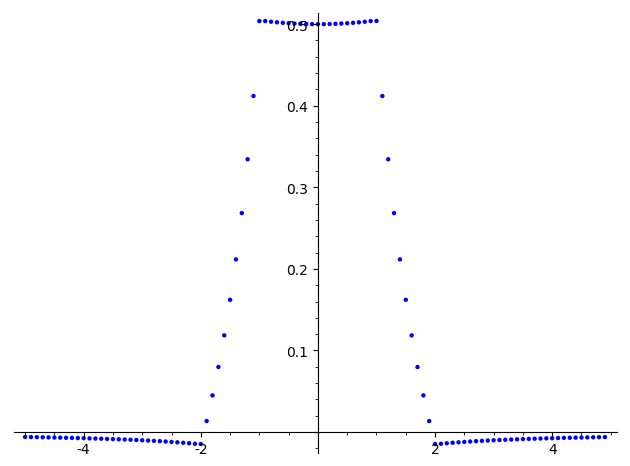
\includegraphics[scale=0.3]{spherical_oscillator_phi_Rneg=2_Rpos=1_v0neg=1_v0pos=0_5_a0neg=0_a0pos=0c=3_t=0}
    \caption{Скалярный потенциал сферического осциллятора (разлёт обкладок)}
    \label{fig:spherical_oscillator_phi_Rneg=2_Rpos=1_v0neg=1_v0pos=0_5_a0neg=0_a0pos=0c=3_t=0}
\end{wrapfigure}

Результат расчёта по формуле  скалярного потенциала Лиенара Вихерта c учётом запаздывания сферического конденсатора, в котором обе обкладки - как внешняя отрицательная  так и внутренняя положительная разлетаются наружу. Скорости обкладок ${{v}_{-}}={}^{1}/{}_{3}c$ и${{v}_{+}}={}^{1}/{}_{6}c$. Начальная фаза центрально-симметричного взрыва. Расчёт проводился для момента времени наблюдения $t=0$.

\begin{wrapfigure}{r}{0.6\textwidth}
    \centering
    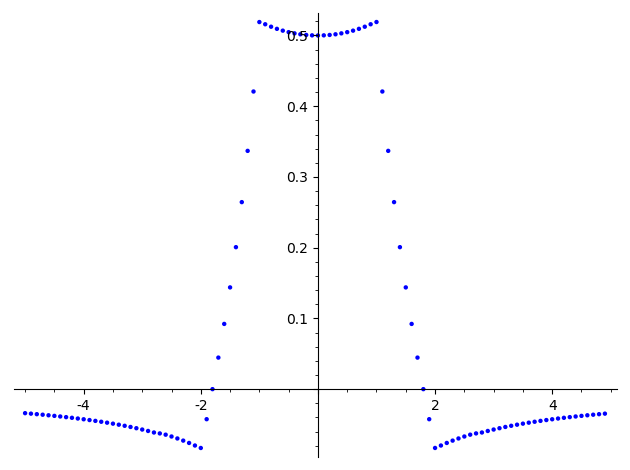
\includegraphics[scale=0.3]{spherical_oscillator_phi_Rneg=2_Rpos=1_v0neg=-2_v0pos=1_a0neg=0_a0pos=0c=3_t=0}
    \caption{Скалярный потенциал сферического осциллятор (схлопывание обкладок t = 0}
    \label{fig:spherical_oscillator_phi_Rneg=2_Rpos=1_v0neg=-2_v0pos=1_a0neg=0_a0pos=0c=3_t=0}
\end{wrapfigure}

Таким образом учёт запаздывания для начальной фазы центрально симметричного взрыва даёт ненулевой градиент скалярного потенциала за пределами его обкладок, как будто внутри сферического конденсатора «образуется унитарный отрицательный заряд», что в принципе уже начинает соответствовать результатам опыта Менде.

\begin{wrapfigure}{l}{0.6\textwidth}
    \centering
    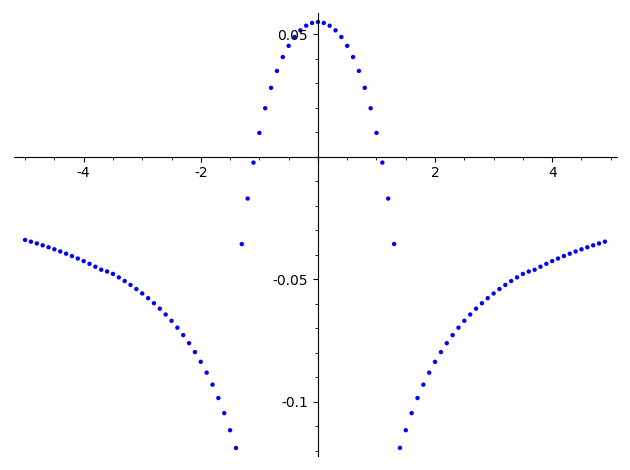
\includegraphics[scale=0.3]{spherical_oscillator_phi_Rneg=2_Rpos=1_v0neg=-2_v0pos=1_a0neg=0_a0pos=0c=3_t=0_3}
    \caption{Скалярный потенциал сферического осциллятор (схлопывание обкладок t = 0.3}
    \label{fig:spherical_oscillator_phi_Rneg=2_Rpos=1_v0neg=-2_v0pos=1_a0neg=0_a0pos=0c=3_t=0_3}
\end{wrapfigure}

Скалярный потенциал Лиенара Вихерта c учётом и без учёта запаздывания сферического конденсатора, в котором положительная обкладка разлетается наружу, а отрицательная обкладка схлопывается внутрь. Обе обкладки движутся навстречу друг другу. Скорости обкладок ${{v}_{-}}=-{}^{2}/{}_{3}c$ и ${{v}_{+}}={}^{1}/{}_{3}c$.

Радиальная компонента векторного потенциала сферически симметричного облака радиально движущихся заряженных частиц на оси $z$ в точке на расстоянии ${{R}_{0}}$ от центра сферы рассчитывается аналогично формуле  с добавлением в числителе интеграла множителя \[{{v}_{r}}\left( t'\left( t,{{r}_{0}},{{v}_{0}},{{a}_{0}},{{R}_{0}},\theta  \right),{{v}_{0}},{{a}_{0}} \right)\cos \theta \] выражающего проекцию скорости частицы в запаздывающий момент времени на ось $z$ 
	\[{{A}_{{{R}_{0}}}}=\int_{{{r}_{0}}}{\left( \frac{\rho \left( {{r}_{0}} \right)}{2}\int\limits_{\theta =0}^{\pi }{\frac{{{v}_{r}}\left( t'\left( t,{{r}_{0}},{{v}_{0}},{{a}_{0}},{{R}_{0}},\theta  \right),{{v}_{0}},{{a}_{0}} \right)\cos \theta \sin \theta d\theta }{{{R}^{*}}\left( t'\left( t,{{r}_{0}},{{v}_{0}},{{a}_{0}},{{R}_{0}},\theta  \right),{{r}_{0}},{{v}_{0}},{{a}_{0}},{{R}_{0}},\theta  \right)}} \right)}d{{r}_{0}}\] 	

Электрическое поле находят из потенциалов Лиенара Вихерта, как известно, дифференцированием скалярного потенциала ЛВ по координатам точки наблюдения и дифференцированием векторного потенциала по времени. Опуская громоздкие промежуточные выкладки, которые можно увидеть, например, здесь (rustot5, n.d.), для градиента по координатам наблюдения скалярного потенциала ЛВ можно привести
	\[\nabla \varphi =\nabla \frac{dq}{{{R}^{*}}}=-\frac{dq}{{{R}^{*}}^{2}}\left\{ \frac{\overrightarrow{R}}{{{R}^{*}}}\left( 1+\frac{\overrightarrow{a}\cdot \overrightarrow{R}}{{{c}^{2}}}-\frac{\overrightarrow{v}\cdot \overrightarrow{v}}{{{c}^{2}}} \right)-\frac{\overrightarrow{v}}{c} \right\}\] 	

А для производной по времени наблюдения векторного потенциала 
	\[\frac{1}{c}\frac{\partial }{\partial t}\overrightarrow{A}=\frac{1}{c}\frac{\partial }{\partial t}\frac{dq\overrightarrow{v}}{c{{R}^{*}}}=\frac{dq}{{{R}^{*}}^{2}}\left\{ \frac{\overrightarrow{a}R}{{{c}^{2}}}-\frac{\overrightarrow{v}}{c}\left( \frac{R}{{{R}^{*}}}\left( -1-\frac{\overrightarrow{a}\cdot \overrightarrow{R}}{{{c}^{2}}}+\frac{\overrightarrow{v}\cdot \overrightarrow{v}}{{{c}^{2}}} \right)+1 \right) \right\}\] 	
где ${{R}^{*}}=\left( R-\frac{\overrightarrow{v}\cdot \overrightarrow{R}}{c} \right)$ - радиус Лиенара Вихерта.

Суммарное электрическое поле
%  $\vec{E} = \frac{q}{k^3}((\vec{r}-\frac{r}{c}\vec{v})(1 + \frac{\vec{r}\vec{a}}{c^2} - \frac{v^2}{c^2}) - \vec{a}\frac{kr}{c^2})$
% http://www.sciteclibrary.ru/cgi-bin/yabb2/YaBB.pl?num=1528093569/415\#415

$$\vec{dE} = \frac{dq}{{{R}^{*}}^{3}}\left( \left(\vec{R}-\frac{R}{c}\vec{v} \right) \left(1 + \frac{\vec{R}\vec{a}}{c^2} - \frac{v^2}{c^2} \right) - \vec{a}\,\frac{{R}^{*}R}{c^2} \right)$$


Для нахождения обоих компонент электрического поля, а также их суммы в точке наблюдения, создаваемого сферой радиально движущихся заряженных частиц, необходимо: во-первых, записать выражение для нормальной ($z$) компоненты электрического поля в точке наблюдения и во-вторых проинтегрировать формулы по сферической поверхности источников поля.

Как видно из вышеприведенных формул вектор электрического поля в точке наблюдения имеет векторные слагаемые со направленные: 1) направлению движения заряда (векторы скорости и ускорения), 2) направлению запаздывающего радиус-вектора (вектора из запаздывающего положения заряда в точку наблюдения).

Для нахождения нормальной компоненты электрического поля в точке наблюдения необходимо: 1) компоненты поля, со направленные скорости и ускорению умножить на косинус зенитного угла $\theta$ источников поля в сферической системе координат, 2) компоненты поля со направленные запаздывающему радиус вектору умножить на косинус угла между запаздывающим радиус-вектором и радиус-вектором из центра сферы в точку наблюдения.

 $$\cos \left( \alpha  \right)'=\frac{\overrightarrow{{{R}_{0}}}\cdot \overrightarrow{R'}}{{{R}_{0}}R'}$$

Учитывая что $\overrightarrow{R'}=-x'\widehat{i}-y'\widehat{j}+\left( {{R}_{0}}-z' \right)\widehat{k}$ а  $\overrightarrow{{{R}_{0}}}={{R}_{0}}\widehat{k}$ тогда $\overrightarrow{{{R}_{0}}}\cdot \overrightarrow{R'}={{R}_{0}}\left( {{R}_{0}}-z' \right)={{R}_{0}}\left( {{R}_{0}}-r'\cos \left( \theta  \right) \right)$ и в итоге
	$$\cos \left( \alpha  \right)'={\left( {{R}_{0}}-r\left( t',{{r}_{0}},{{v}_{0}},{{a}_{0}} \right)\cos \left( \theta  \right) \right)}/{R'}\;$$

Скалярное произведение ускорения частицы в запаздывающий момент времени на запаздывающий радиус-вектор (вектор из запаздывающего положения заряда в точку наблюдения), по аналогии с формулой скалярного произведения вектора радиальной скорости частиц на запаздывающий радиус-вектор
	\[\left( \overrightarrow{a}\cdot \overrightarrow{R} \right)'=a'\left( {{R}_{0}}\cos \theta -r\left( t',{{r}_{0}},{{v}_{0}},{{a}_{0}} \right) \right)\] 	

Первое слагаемое радиальной компоненты электрического поля, вычисляемое как минус градиент скалярного потенциала, можно выразить подставляя  в  , при этом для нахождения радиальной проекции вектора запаздывающего радиуса его модуль умножается на  таким образом${{\left( \overrightarrow{R'} \right)}_{{{R}_{0}}}}=R'\cos \left( \alpha  \right)'$ , а для нахождения радиальной (то есть $z$) компоненты вектора запаздывающей скорости, ее модуль умножается на 
	\[d{{E}_{1}}=-{{\left( \nabla \varphi  \right)}_{{{R}_{0}}}}=\frac{dq}{{{R}^{*}}^{2}}\left\{ \frac{R'\cos \left( \alpha  \right)'}{{{R}^{*}}}\left( 1+\frac{\left( \overrightarrow{a}\cdot \overrightarrow{R} \right)'}{{{c}^{2}}}-\frac{\overrightarrow{v'}\cdot \overrightarrow{v'}}{{{c}^{2}}} \right)-\frac{v'\cos \left( \theta  \right)}{c} \right\}\]

Аналогично, из формулы  выражается второе слагаемое радиальной компоненты электрического поля. Здесь для получения проекций запаздывающих векторов скорости и ускорения их модули умножаются на $\cos \left( \theta  \right)$

	\[d{{E}_{2}}=-\frac{1}{c}{{\left( \frac{\partial }{\partial t}\overrightarrow{A} \right)}_{{{R}_{0}}}}=\]

\[\frac{dq\cos \left( \theta  \right)}{{{R}^{*}}^{2}}\left\{ \frac{v'}{c}\left( \frac{R}{{{R}^{*}}}\left( -1-\frac{\left( \overrightarrow{a}\cdot \overrightarrow{R} \right)'}{{{c}^{2}}}+\frac{\overrightarrow{v}\cdot \overrightarrow{v}}{{{c}^{2}}} \right)+1 \right)-\frac{a'R}{{{c}^{2}}} \right\}\] 

Радиальная компонента суммарного электрического поля

$$dE = \frac{dq}{{{R}^{*}}^{3}} \left( \left({R'\cos \left( \alpha  \right)'}-\frac{R'}{c}{v'\cos \left( \theta  \right)} \right) \left(1 + \frac{\vec{R}\vec{a}}{c^2} - \frac{v^2}{c^2} \right) - {a' \cos \left( \theta  \right)}\frac{{R}^{*}R'}{c^2} \right)$$

% Подставляя выражения для $R'=c\left( t-t' \right)$ и $\cos \left( \alpha  \right)'$


% $$\vec{dE} = \frac{dq}{{{R}^{*}}^{3}} \left( \left({R}_{0}-r \left( t' \right)\cos \left( \theta  \right) - \left( t-t' \right) {v'\cos \left( \theta  \right)} \right) \left(1 + \frac{\vec{R}\vec{a}}{c^2} - \frac{v^2}{c^2} \right) - {a' \cos \left( \theta  \right)}\frac{{R}^{*}\left( t-t' \right)}{c} \right)$$

% $$\overrightarrow{dE}=\frac{dq}{{{R}^{*}}^{3}}\left( \left( {{R}_{0}}-\left( r\left( {{t}'} \right)+\left( t-{t}' \right){v}' \right)\cos \left( \theta  \right) \right)\left( 1+\frac{\vec{R}\vec{a}}{{{c}^{2}}}-\frac{{{v}^{2}}}{{{c}^{2}}} \right)-{a}'\cos \left( \theta  \right)\frac{{{R}^{*}}\left( t-{t}' \right)}{c} \right)$$

%$$\frac{dE}{dq}=\frac{\left( {{R}_{0}}-\left( r\left( {{t}'} \right)+\left( t-{t}' \right)v\left( {{t}'} \right) \right)\cos \left( \theta  \right) \right)}{{{R}^{*}}^{3}}\left( 1+\frac{\vec{R}\vec{a}}{{{c}^{2}}}-\frac{{{v}^{2}}}{{{c}^{2}}} \right)-a\left( {{t}'} \right)\cos \left( \theta  \right)\frac{\left( t-{t}' \right)}{c{{R}^{*}}^{2}}$$

%подставляя выражение для $\vec{R}\vec{a}=a\left( {{t}'} \right)\left( {{R}_{0}}\cos \theta -r\left( t' \right) \right)$


%$$\frac{dE}{dq}=\frac{\left( {{R}_{0}}-\left( r+\left( t-{t}' \right)v \right)\cos \left( \theta  \right) \right)}{{{R}^{*}}^{3}}\left( 1+\frac{a\left( {{R}_{0}}\cos \theta -r \right)}{{{c}^{2}}}-\frac{{{v}^{2}}}{{{c}^{2}}} \right)-a\cos \left( \theta  \right)\frac{\left( t-{t}' \right)}{c{{R}^{*}}^{2}}$$

В данном выражении величины $r$, $v$ и $a$, зависящие от координаты $\theta$ источника поля вычисляются для запаздывающего момента времени $t'$.

Радиус Лиенара Вихерта в сферической системе координат через запаздывающий момент вычисляется как

\[{{R}^{*}}=c\left( t-t' \right)-\frac{v}{c}\left( {{R}_{0}}\cos \theta -r \right)\]

Слагающая электрического поля, создаваемая эффектом разлёта заряженных частиц для сферического конденсатора вычисляется интегрированием по углу  принимая для  заряд обкладки и вынося его за знак интегрирования

	\[E=\int\limits_{S}{\left( \frac{d{{E}_{1}}}{dq}+\frac{d{{E}_{2}}}{dq} \right)\ }\sigma dS=\frac{q}{2}\int\limits_{0}^{\pi }{\left( \frac{d{{E}_{1}}}{dq}+\frac{d{{E}_{2}}}{dq} \right)}\ \sin \theta d\theta \]

А для объёмного случая
	\[E=\int_{{{r}_{0}}}{\left( \frac{\rho \left( {{r}_{0}} \right)}{2}\int\limits_{\theta =0}^{\pi }{\left( \frac{d{{E}_{1}}}{dq}+\frac{d{{E}_{2}}}{dq} \right)\sin \theta d\theta } \right)}\ d{{r}_{0}}\]
где ${\rho \left( {{r}_{0}} \right)=\partial q}/{\partial {{r}_{0}}}\;$- радиальная (не объёмная!) плотность заряда, то есть отношение заряда в объёме между концентрическими сферами близких радиусов к разности радиусов этих сфер.

Проводя аналогию с формулой закона Кулона (Тамм, 1957), [3]
	\[\overrightarrow{E}=\frac{q}{{{R}^{3}}} \overrightarrow{R}\] \[E=\frac{q}{{{R}^{2}}}\]

Вычислив электрическое поле по формулам  – для сферического конденсатора или  – для объёмного взрыва, можно оценить величину так называемого «дополнительного заряда».
% Расчёт тока смещения в модели центрально-симметричного взрыва
% Численный расчёт методом конечных разностей по формулам ,  и так далее чреват возникновением численных неустойчивостей поэтому возникает необходимость учёта производных по времени электрических полей ${{E}_{1}}$ и ${{E}_{2}}$

% \[\overrightarrow{{{E}_{1}}}=-\nabla \varphi =-\nabla \frac{q}{{{R}^{*}}}=\frac{q}{{{R}^{*}}^{2}}\left\{ \frac{\overrightarrow{R}}{{{R}^{*}}}\left( 1+\frac{\overrightarrow{a}\cdot \overrightarrow{R}}{{{c}^{2}}}-\frac{\overrightarrow{v}\cdot \overrightarrow{v}}{{{c}^{2}}} \right)-\frac{\overrightarrow{v}}{c} \right\}\]

% Записываем выражение для производной по времени
% \[\frac{1}{q}\frac{\partial \overrightarrow{{{E}_{1}}}}{\partial t}= \]

% \[\frac{\partial }{\partial t}\left[ \frac{\overrightarrow{R}}{{{R}^{*}}^{3}}\left( 1+\frac{\overrightarrow{a}\cdot \overrightarrow{R}}{{{c}^{2}}}-\frac{\overrightarrow{v}\cdot \overrightarrow{v}}{{{c}^{2}}} \right)-\frac{1}{{{R}^{*}}^{2}}\frac{\overrightarrow{v}}{c} \right]=\]

% \[\frac{\overrightarrow{R}}{{{R}^{*}}^{3}}\frac{\partial }{\partial t}\left( \frac{\overrightarrow{a}\cdot \overrightarrow{R}}{{{c}^{2}}}-\frac{\overrightarrow{v}\cdot \overrightarrow{v}}{{{c}^{2}}} \right)+\left( 1+\frac{\overrightarrow{a}\cdot \overrightarrow{R}}{{{c}^{2}}}-\frac{\overrightarrow{v}\cdot \overrightarrow{v}}{{{c}^{2}}} \right)\cdot \frac{\partial }{\partial t}\left( \frac{\overrightarrow{R}}{{{R}^{*}}^{3}} \right)-\frac{\partial }{\partial t}\left( \frac{1}{{{R}^{*}}^{2}}\frac{\overrightarrow{v}}{c} \right)\] 
% Первую промежуточную производную можно представить как

% \[\frac{\partial }{\partial t}\left( \frac{\overrightarrow{a}\cdot \overrightarrow{R}}{{{c}^{2}}}-\frac{\overrightarrow{v}\cdot \overrightarrow{v}}{{{c}^{2}}} \right)=\frac{1}{{{c}^{2}}}\frac{\partial }{\partial t}\left( \overrightarrow{a}\cdot \overrightarrow{R}-\overrightarrow{v}\cdot \overrightarrow{v} \right)=\frac{1}{{{c}^{2}}}\left( \overrightarrow{a}\frac{\partial \overrightarrow{R}}{\partial t}+\overrightarrow{R}\frac{\partial \overrightarrow{a}}{\partial t}-2\overrightarrow{v}\frac{\partial \overrightarrow{v}}{\partial t} \right)=\frac{1}{{{c}^{2}}}\left( \overrightarrow{a}\frac{\partial \overrightarrow{R}}{\partial t'}+\overrightarrow{R}\frac{\partial \overrightarrow{a}}{\partial t'}-2\overrightarrow{v}\frac{\partial \overrightarrow{v}}{\partial t'} \right)\frac{\partial t'}{\partial t}\]
% Далее
% \[\frac{\partial }{\partial t}\left( \frac{\overrightarrow{a}\cdot \overrightarrow{R}}{{{c}^{2}}}-\frac{\overrightarrow{v}\cdot \overrightarrow{v}}{{{c}^{2}}} \right)=\frac{1}{{{c}^{2}}}\frac{R}{{{R}^{*}}}\left( -\,\overrightarrow{a}\cdot \overrightarrow{v}+\overrightarrow{R}\frac{\partial \overrightarrow{a}}{\partial t'}-2\overrightarrow{v}\cdot \overrightarrow{a} \right)=\frac{1}{{{c}^{2}}}\frac{R}{{{R}^{*}}}\left( \overrightarrow{R}\frac{\partial \overrightarrow{a}}{\partial t'}-3\ \overrightarrow{v}\cdot \overrightarrow{a} \right)\]
% Вторая промежуточная производная
% \[\frac{\partial }{\partial t}\left( \frac{\overrightarrow{R}}{{{R}^{*}}^{3}} \right)=\frac{1}{{{R}^{*}}^{3}}\frac{\partial \overrightarrow{R}}{\partial t}+\overrightarrow{R}\frac{\partial }{\partial t}\left( \frac{1}{{{R}^{*}}^{3}} \right)=\frac{1}{{{R}^{*}}^{3}}\frac{\partial \overrightarrow{R}}{\partial t'}\frac{\partial t'}{\partial t}-\frac{3\overrightarrow{R}}{{{R}^{*}}^{4}}\frac{\partial {{R}^{*}}}{\partial t}=-\frac{\overrightarrow{v}}{{{R}^{*}}^{3}}\frac{R}{{{R}^{*}}}-\frac{3\overrightarrow{R}}{{{R}^{*}}^{4}}\frac{\partial {{R}^{*}}}{\partial t'}\frac{\partial t'}{\partial t}=-\frac{\overrightarrow{v}R}{{{R}^{*}}^{4}}-\frac{3\overrightarrow{R}R}{{{R}^{*}}^{5}}\frac{\partial {{R}^{*}}}{\partial t'}\]
% Поскольку
% \[\frac{\partial {{R}^{*}}}{\partial t'}=\frac{\partial }{\partial t'}\left( R-\frac{\overrightarrow{v}\cdot \overrightarrow{R}}{c} \right)=\frac{\overrightarrow{v}\cdot \overrightarrow{v}-\overrightarrow{R}\cdot \overrightarrow{a}}{c}-\frac{\overrightarrow{R}\cdot \overrightarrow{v}}{R}\]
% тогда
% \[\frac{\partial }{\partial t}\left( \frac{\overrightarrow{R}}{{{R}^{*}}^{3}} \right)=-\frac{\overrightarrow{v}R}{{{R}^{*}}^{4}}-\frac{3\overrightarrow{R}R}{{{R}^{*}}^{5}}\left( \frac{\overrightarrow{v}\cdot \overrightarrow{v}-\overrightarrow{R}\cdot \overrightarrow{a}}{c}-\frac{\overrightarrow{R}\cdot \overrightarrow{v}}{R} \right)\]
% Третья промежуточная производная
% \[\frac{\partial }{\partial t}\left( \frac{1}{{{R}^{*}}^{2}}\frac{\overrightarrow{v}}{c} \right)=\frac{\overrightarrow{v}}{c}\frac{\partial }{\partial t}\left( \frac{1}{{{R}^{*}}^{2}} \right)+\frac{1}{{{R}^{*}}^{2}}\frac{\partial }{\partial t}\left( \frac{\overrightarrow{v}}{c} \right)=\left( -\frac{2}{{{R}^{*}}^{3}}\frac{\overrightarrow{v}}{c}\frac{\partial {{R}^{*}}}{\partial t'}+\frac{1}{c{{R}^{*}}^{2}}\frac{\partial \overrightarrow{v}}{\partial t'} \right)\frac{\partial t'}{\partial t}=\left\{ -\frac{2}{{{R}^{*}}^{3}}\frac{\overrightarrow{v}}{c}\left( \frac{\overrightarrow{v}\cdot \overrightarrow{v}-\overrightarrow{R}\cdot \overrightarrow{a}}{c}-\frac{\overrightarrow{R}\cdot \overrightarrow{v}}{R} \right)+\frac{\overrightarrow{a}}{c{{R}^{*}}^{2}} \right\}\frac{R}{{{R}^{*}}}\]
% Подставляя
% \[\frac{1}{q}\frac{\partial \overrightarrow{{{E}_{1}}}}{\partial t}= \]

% \[\frac{\overrightarrow{R}}{{{R}^{*}}^{3}}\frac{1}{{{c}^{2}}}\frac{R}{{{R}^{*}}}\left( \overrightarrow{R}\frac{\partial \overrightarrow{a}}{\partial t'}-3\ \overrightarrow{v}\cdot \overrightarrow{a} \right)-\left( 1+\frac{\overrightarrow{a}\cdot \overrightarrow{R}}{{{c}^{2}}}-\frac{\overrightarrow{v}\cdot \overrightarrow{v}}{{{c}^{2}}} \right)\cdot \left\{ \frac{\overrightarrow{v}R}{{{R}^{*}}^{4}}+\frac{3\overrightarrow{R}R}{{{R}^{*}}^{5}}\left( \frac{\overrightarrow{v}\cdot \overrightarrow{v}-\overrightarrow{R}\cdot \overrightarrow{a}}{c}-\frac{\overrightarrow{R}\cdot \overrightarrow{v}}{R} \right) \right\}+ \\ 
%   +\left\{ \frac{2}{{{R}^{*}}^{3}}\frac{\overrightarrow{v}}{c}\left( \frac{\overrightarrow{v}\cdot \overrightarrow{v}-\overrightarrow{R}\cdot \overrightarrow{a}}{c}-\frac{\overrightarrow{R}\cdot \overrightarrow{v}}{R} \right)-\frac{\overrightarrow{a}}{c{{R}^{*}}^{2}} \right\}\frac{R}{{{R}^{*}}} \\ 
% \]
% Вторая компонента электрического поля – вихревое электрическое поле, оно же поле электромагнитной индукции
%\[{{E}_{2}}=-\frac{1}{c}\frac{\partial }{\partial t}\overrightarrow{A}=\frac{q}{{{R}^{*}}^{2}}\left\{ \frac{\overrightarrow{v}}{c}\left( \frac{R}{{{R}^{*}}}\left( \frac{\overrightarrow{v}\cdot \overrightarrow{v}}{{{c}^{2}}}-\frac{\overrightarrow{a}\cdot \overrightarrow{R}}{{{c}^{2}}}-1 \right)+1 \right)-\frac{\overrightarrow{a}R}{{{c}^{2}}} \right\}\]
% Записываем выражение производной по времени
% \[\frac{1}{q}\frac{\partial {{E}_{2}}}{\partial t}=\left\{ \frac{\overrightarrow{v}}{c}\left( \frac{R}{{{R}^{*}}}\left( \frac{\overrightarrow{v}\cdot \overrightarrow{v}}{{{c}^{2}}}-\frac{\overrightarrow{a}\cdot \overrightarrow{R}}{{{c}^{2}}}-1 \right)+1 \right)-\frac{\overrightarrow{a}R}{{{c}^{2}}} \right\}\frac{\partial }{\partial t}\left( \frac{1}{{{R}^{*}}^{2}} \right)+\frac{1}{{{R}^{*}}^{2}}\frac{\partial }{\partial t}\left( \frac{\overrightarrow{v}}{c}\frac{R}{{{R}^{*}}}\frac{\overrightarrow{v}\cdot \overrightarrow{v}}{{{c}^{2}}}-\frac{\overrightarrow{v}}{c}\frac{R}{{{R}^{*}}}\frac{\overrightarrow{a}\cdot \overrightarrow{R}}{{{c}^{2}}}-\frac{\overrightarrow{v}}{c}\frac{R}{{{R}^{*}}}+\frac{\overrightarrow{v}}{c}-\frac{\overrightarrow{a}R}{{{c}^{2}}} \right)\]
% Первая промежуточная производная равна
% \[\frac{\partial }{\partial t}\left( \frac{1}{{{R}^{*}}^{2}} \right)=-\frac{2}{{{R}^{*}}^{3}}\frac{\partial {{R}^{*}}}{\partial t}=-\frac{2}{{{R}^{*}}^{3}}\frac{\partial {{R}^{*}}}{\partial t'}\frac{\partial t'}{\partial t}=-\frac{2}{{{R}^{*}}^{3}}\left( \frac{\overrightarrow{v}\cdot \overrightarrow{v}-\overrightarrow{R}\cdot \overrightarrow{a}}{c}-\frac{\overrightarrow{R}\cdot \overrightarrow{v}}{R} \right)\frac{R}{{{R}^{*}}}\]
% Вторая промежуточная производная
% \[\frac{\partial }{\partial t}\left( \frac{\overrightarrow{v}}{c}\frac{R}{{{R}^{*}}}\frac{\overrightarrow{v}\cdot \overrightarrow{v}}{{{c}^{2}}} \right)=\frac{\overrightarrow{v}\cdot \overrightarrow{v}}{{{c}^{2}}}\frac{\partial }{\partial t}\left( \frac{\overrightarrow{v}}{c}\frac{R}{{{R}^{*}}} \right)+\frac{\overrightarrow{v}}{c}\frac{R}{{{R}^{*}}}\frac{\partial }{\partial t}\left( \frac{\overrightarrow{v}\cdot \overrightarrow{v}}{{{c}^{2}}} \right)\]
% \[\frac{\partial }{\partial t}\left( \frac{\overrightarrow{v}\cdot \overrightarrow{v}}{{{c}^{2}}} \right)=\frac{2R}{{{R}^{*}}}\frac{\overrightarrow{v}\cdot \overrightarrow{a}}{{{c}^{2}}}\]
% \[\frac{\partial }{\partial t}\left( \frac{\overrightarrow{v}}{c}\frac{R}{{{R}^{*}}} \right)=\frac{R}{c{{R}^{*}}}\left( \overrightarrow{a}\frac{R}{{{R}^{*}}}-\overrightarrow{v}\left( \frac{R}{{{R}^{*}}^{2}}\left( \frac{\overrightarrow{v}\cdot \overrightarrow{v}-\overrightarrow{R}\cdot \overrightarrow{a}}{c}-\frac{\overrightarrow{R}\cdot \overrightarrow{v}}{R} \right)+\frac{\overrightarrow{R}\cdot \overrightarrow{v}}{R} \right) \right)\]
% \[\frac{\partial }{\partial t}\left( \frac{\overrightarrow{v}}{c}\frac{R}{{{R}^{*}}}\frac{\overrightarrow{v}\cdot \overrightarrow{v}}{{{c}^{2}}} \right)=\frac{\overrightarrow{v}\cdot \overrightarrow{v}}{{{c}^{2}}}\left\{ \frac{R}{c{{R}^{*}}}\left( \overrightarrow{a}\frac{R}{{{R}^{*}}}-\overrightarrow{v}\left( \frac{R}{{{R}^{*}}^{2}}\left( \frac{\overrightarrow{v}\cdot \overrightarrow{v}-\overrightarrow{R}\cdot \overrightarrow{a}}{c}-\frac{\overrightarrow{R}\cdot \overrightarrow{v}}{R} \right)+\frac{\overrightarrow{R}\cdot \overrightarrow{v}}{R} \right) \right) \right\}+\frac{\overrightarrow{v}}{c}\frac{R}{{{R}^{*}}}\frac{2R}{{{R}^{*}}}\frac{\overrightarrow{v}\cdot \overrightarrow{a}}{{{c}^{2}}}\]
% Третья промежуточная производная
% \[\frac{\partial }{\partial t}\left( -\frac{\overrightarrow{v}}{c}\frac{R}{{{R}^{*}}}\frac{\overrightarrow{a}\cdot \overrightarrow{R}}{{{c}^{2}}} \right)=-\frac{\overrightarrow{a}\cdot \overrightarrow{R}}{{{c}^{2}}}\frac{\partial }{\partial t}\left( \frac{\overrightarrow{v}}{c}\frac{R}{{{R}^{*}}} \right)-\frac{\overrightarrow{v}}{c}\frac{R}{{{R}^{*}}}\frac{\partial }{\partial t}\left( \frac{\overrightarrow{a}\cdot \overrightarrow{R}}{{{c}^{2}}} \right)\]
% \[\frac{\partial }{\partial t}\left( \frac{\overrightarrow{a}\cdot \overrightarrow{R}}{{{c}^{2}}} \right)=\frac{1}{{{c}^{2}}}\frac{R}{{{R}^{*}}}\left( -\,\overrightarrow{a}\cdot \overrightarrow{v}+\overrightarrow{R}\frac{\partial \overrightarrow{a}}{\partial t'} \right)\]

%\[\frac{\partial }{\partial t}\left( -\frac{\overrightarrow{v}}{c}\frac{R}{{{R}^{*}}}\frac{\overrightarrow{a}\cdot \overrightarrow{R}}{{{c}^{2}}} \right)=-\frac{\overrightarrow{a}\cdot \overrightarrow{R}}{{{c}^{2}}}\left\{ \frac{R}{c{{R}^{*}}}\left( \overrightarrow{a}\frac{R}{{{R}^{*}}}-\overrightarrow{v}\left( \frac{R}{{{R}^{*}}^{2}}\left( \frac{\overrightarrow{v}\cdot \overrightarrow{v}-\overrightarrow{R}\cdot \overrightarrow{a}}{c}-\frac{\overrightarrow{R}\cdot \overrightarrow{v}}{R} \right)+\frac{\overrightarrow{R}\cdot \overrightarrow{v}}{R} \right) \right) \right\}-\frac{\overrightarrow{v}}{c}\frac{R}{{{R}^{*}}}\frac{1}{{{c}^{2}}}\frac{R}{{{R}^{*}}}\left( -\,\overrightarrow{a}\cdot \overrightarrow{v}+\overrightarrow{R}\frac{\partial \overrightarrow{a}}{\partial t'} \right)\]

% Четвертая промежуточная производная

% \[\frac{\partial }{\partial t}\left( -\frac{\overrightarrow{v}}{c}\frac{R}{{{R}^{*}}} \right)=-\frac{1}{c}\frac{\partial }{\partial t}\left( \overrightarrow{v}\frac{R}{{{R}^{*}}} \right)=-\frac{1}{c}\frac{\partial }{\partial t'}\left( \overrightarrow{v}\frac{R}{{{R}^{*}}} \right)\frac{\partial t'}{\partial t}=-\frac{R}{c{{R}^{*}}}\left( \overrightarrow{a}\frac{R}{{{R}^{*}}}+\overrightarrow{v}\frac{\partial }{\partial t'}\left( \frac{R}{{{R}^{*}}} \right) \right)\]
% \[\frac{\partial R}{\partial t'}=\frac{\partial }{\partial t'}{{\left( \overrightarrow{R}\cdot \overrightarrow{R} \right)}^{{}^{1}/{}_{2}}}=\frac{1}{2}{{\left( \overrightarrow{R}\cdot \overrightarrow{R} \right)}^{-{}^{1}/{}_{2}}}\frac{\partial }{\partial t'}\left( \overrightarrow{R}\cdot \overrightarrow{R} \right)=\frac{1}{2R}\left( \overrightarrow{R}\cdot \frac{\partial \overrightarrow{R}}{\partial t'}+\frac{\partial \overrightarrow{R}}{\partial t'}\cdot \overrightarrow{R} \right)=\frac{\overrightarrow{R}}{R}\cdot \frac{\partial \overrightarrow{R}}{\partial t'}=-\frac{\overrightarrow{R}\cdot \overrightarrow{v}}{R}\]
% \[\frac{\partial }{\partial t'}\left( \frac{R}{{{R}^{*}}} \right)=R\frac{\partial }{\partial t'}\left( \frac{1}{{{R}^{*}}} \right)+\frac{1}{{{R}^{*}}}\frac{\partial R}{\partial t'}=-\frac{R}{{{R}^{*}}^{2}}\frac{\partial {{R}^{*}}}{\partial t'}-\frac{\overrightarrow{R}\cdot \overrightarrow{v}}{R}=-\frac{R}{{{R}^{*}}^{2}}\left( \frac{\overrightarrow{v}\cdot \overrightarrow{v}-\overrightarrow{R}\cdot \overrightarrow{a}}{c}-\frac{\overrightarrow{R}\cdot \overrightarrow{v}}{R} \right)-\frac{\overrightarrow{R}\cdot \overrightarrow{v}}{R}\]
% \[\frac{\partial }{\partial t}\left( -\frac{\overrightarrow{v}}{c}\frac{R}{{{R}^{*}}} \right)=-\frac{R}{c{{R}^{*}}}\left( \overrightarrow{a}\frac{R}{{{R}^{*}}}-\overrightarrow{v}\left( \frac{R}{{{R}^{*}}^{2}}\left( \frac{\overrightarrow{v}\cdot \overrightarrow{v}-\overrightarrow{R}\cdot \overrightarrow{a}}{c}-\frac{\overrightarrow{R}\cdot \overrightarrow{v}}{R} \right)+\frac{\overrightarrow{R}\cdot \overrightarrow{v}}{R} \right) \right)\]
% Пятая промежуточная производная
% \[\frac{\partial }{\partial t}\left( \frac{\overrightarrow{v}}{c} \right)=\frac{1}{c}\frac{\partial \overrightarrow{v}}{\partial t'}\frac{\partial t'}{\partial t}=\frac{\overrightarrow{a}}{c}\frac{R}{{{R}^{*}}}\]
% Шестая промежуточная производная
% \[\frac{\partial }{\partial t}\left( -\frac{\overrightarrow{a}R}{{{c}^{2}}} \right)=-\frac{1}{{{c}^{2}}}\frac{\partial }{\partial t'}\left( \overrightarrow{a}R \right)\frac{\partial t'}{\partial t}=-\frac{1}{{{c}^{2}}}\frac{R}{{{R}^{*}}}\left( R\frac{\partial \overrightarrow{a}}{\partial t'}+\overrightarrow{a}\frac{\partial R}{\partial t'} \right)=-\frac{1}{{{c}^{2}}}\frac{R}{{{R}^{*}}}\left( R\frac{\partial \overrightarrow{a}}{\partial t'}-\overrightarrow{a}\frac{\overrightarrow{R}\cdot \overrightarrow{v}}{R} \right)\]
% Итого
% \[
%  & \frac{1}{q}\frac{\partial {{E}_{2}}}{\partial t}=\left\{ \frac{\overrightarrow{v}}{c}\left( \frac{R}{{{R}^{*}}}\left( \frac{\overrightarrow{v}\cdot \overrightarrow{v}}{{{c}^{2}}}-\frac{\overrightarrow{a}\cdot \overrightarrow{R}}{{{c}^{2}}}-1 \right)+1 \right)-\frac{\overrightarrow{a}R}{{{c}^{2}}} \right\}\left\{ -\frac{2}{{{R}^{*}}^{3}}\left( \frac{\overrightarrow{v}\cdot \overrightarrow{v}-\overrightarrow{R}\cdot \overrightarrow{a}}{c}-\frac{\overrightarrow{R}\cdot \overrightarrow{v}}{R} \right)\frac{R}{{{R}^{*}}} \right\} \\ 
% & +\frac{1}{{{R}^{*}}^{2}}\left\{ \frac{\overrightarrow{v}\cdot \overrightarrow{v}}{{{c}^{2}}}\left\{ \frac{R}{c{{R}^{*}}}\left( \overrightarrow{a}\frac{R}{{{R}^{*}}}-\overrightarrow{v}\left( \frac{R}{{{R}^{*}}^{2}}\left( \frac{\overrightarrow{v}\cdot \overrightarrow{v}-\overrightarrow{R}\cdot \overrightarrow{a}}{c}-\frac{\overrightarrow{R}\cdot \overrightarrow{v}}{R} \right)+\frac{\overrightarrow{R}\cdot \overrightarrow{v}}{R} \right) \right) \right\}+\frac{\overrightarrow{v}}{c}\frac{R}{{{R}^{*}}}\frac{2R}{{{R}^{*}}}\frac{\overrightarrow{v}\cdot \overrightarrow{a}}{{{c}^{2}}} \right\} \\ 
% & +\frac{1}{{{R}^{*}}^{2}}\left\{ -\frac{\overrightarrow{a}\cdot \overrightarrow{R}}{{{c}^{2}}}\left\{ \frac{R}{c{{R}^{*}}}\left( \overrightarrow{a}\frac{R}{{{R}^{*}}}-\overrightarrow{v}\left( \frac{R}{{{R}^{*}}^{2}}\left( \frac{\overrightarrow{v}\cdot \overrightarrow{v}-\overrightarrow{R}\cdot \overrightarrow{a}}{c}-\frac{\overrightarrow{R}\cdot \overrightarrow{v}}{R} \right)+\frac{\overrightarrow{R}\cdot \overrightarrow{v}}{R} \right) \right) \right\}-\frac{\overrightarrow{v}}{c}\frac{R}{{{R}^{*}}}\frac{1}{{{c}^{2}}}\frac{R}{{{R}^{*}}}\left( -\,\overrightarrow{a}\cdot \overrightarrow{v}+\overrightarrow{R}\frac{\partial \overrightarrow{a}}{\partial t'} \right) \right\} \\ 
% & +\frac{1}{{{R}^{*}}^{2}}\left\{ -\frac{R}{c{{R}^{*}}}\left( \overrightarrow{a}\frac{R}{{{R}^{*}}}-\overrightarrow{v}\left( \frac{R}{{{R}^{*}}^{2}}\left( \frac{\overrightarrow{v}\cdot \overrightarrow{v}-\overrightarrow{R}\cdot \overrightarrow{a}}{c}-\frac{\overrightarrow{R}\cdot \overrightarrow{v}}{R} \right)+\frac{\overrightarrow{R}\cdot \overrightarrow{v}}{R} \right) \right) \right\} \\ 
% & +\frac{1}{{{R}^{*}}^{2}}\left\{ \frac{\overrightarrow{a}}{c}\frac{R}{{{R}^{*}}} \right\} \\ 
% & +\frac{1}{{{R}^{*}}^{2}}\left\{ -\frac{1}{{{c}^{2}}}\frac{R}{{{R}^{*}}}\left( R\frac{\partial \overrightarrow{a}}{\partial t'}-\overrightarrow{a}\frac{\overrightarrow{R}\cdot \overrightarrow{v}}{R} \right) \right\} \\ 
%\]
\section{Сравнение с результатами эксперимента}

%Подготовка данных к численному итерационному расчёту.

Было бы правильно для моделирования динамики центрально симметричного взрыва плазмы решать дифференциальные уравнения магнитной гидродинамики с учетом теплопередачи, но столь сложное исследование не входит рамки данной работы, поэтому были произведены достаточно грубые оценки предположительных параметров взрыва следующим образом.

Пусть в конце фазы разогрева первоначальная плазма имеет радиус ${{R}_{1}}$ а изначальная плотность частиц равна   \[{{n}_{i}}=\frac{{{N}_{i}}}{\int\limits_{0}^{{{R}_{i}}}{4\pi {{r}^{2}}dr}}=\frac{3{{N}_{i}}}{4\pi {{R}_{1}}^{3}}\]

Для распределения радиальной компоненты скорости частиц примем линейную аппроксимацию в виде: 

	$${{v}_{R}}=\alpha \frac{R}{{{R}_{1}}}{{v}_{T}}$$
	
где ${{v}_{T}}$ средняя тепловая скорость частиц, $\alpha $ коэффициент пропорциональности.

На возможность принятия линейного аппроксимации зависимости скорости частиц от координаты в качестве первого приближения для проведения приближённых оценочных расчётов указывают результаты расчётной работы (Сасакин, 2016).

Принимая в качестве статистики распределения скорости частиц по окончании периода разогрева плазмы распределение Максвелла 

	\[\frac{dN}{d{{v}_{0}}}=N{{\left[ \frac{m}{2\pi kT} \right]}^{{}^{3}/{}_{2}}}{{v}^{2}}\exp \left( -\frac{m{{v}^{2}}}{2kT} \right)\]


Получаем  среднюю тепловую скорость частиц  ${{v}_{T}}=\sqrt{\frac{2{{k}_{B}}T}{m}}$ откуда
	${{v}_{R}}=\alpha \frac{R}{{{R}_{1}}}\sqrt{\frac{2{{k}_{B}}T}{m}}$

Для распределения радиальной компоненты начальной скорости частиц будем исходить из следующих соображений - в поверхностном слое взрывающегося шара средняя тепловая скорость частиц наиболее полно превращается в радиальную скорость за счёт отражения от приповерхностного слоя частиц и за счёт отсутствия препятствий (если пренебречь сопротивлением воздуха или производить взрыв в вакууме) с внешней стороны взрывающегося шара.

Для нахождения коэффициента преобразования средней тепловой скорости частиц в радиальную для поверхностного слоя взрывающегося шара достаточно проинтегрировать косинус зенитного угла $\theta$ по полусфере направлений скоростей в сферической системе координат

$\alpha =\frac{\int\limits_{0}^{\pi /2}{r\int\limits_{0}^{2\pi }{r\ \sin \left( \theta  \right)d\varphi \cos \left( \theta  \right)d\theta }}}{\int\limits_{0}^{\pi /2}{r\int\limits_{0}^{2\pi }{r\ \sin \left( \theta  \right)d\varphi d\theta }}}$

%phi = var("phi")
%half_sphere_S                   = integrate(r*integrate(r*sin(theta), (phi, 0, 2*pi))                   ,(theta, 0, pi/2))
%half_sphere_S_cos_theta = integrate(r*integrate(r*sin(theta), (phi, 0, 2*pi))*cos(theta),(theta, 0, pi/2))
%alpha = half_sphere_S_cos_theta / half_sphere_S
%print ("alpha = ", alpha)
%print ("should be 1/2")

Исходя из этих соображений принимаем в распределении радиальной компоненты скорости частиц коэффициент пропорциональности равным $$\alpha = 0.5$$


В описании своего опыта в работе «Является ли заряд инвариантом скорости?» (Менде, Является ли заряд инвариантом скорости?, 2015) приводит следующие данные

“Если посчитать энергию, необходимую для разогрева, плавления и испарения медной проволоки диаметром 0.2 мм и длиной 5 мм то она составит около 8 Дж. При этом температура паров меди уже будет составлять около 2800 К. Энергия же конденсатора ёмкостью 3000 мкФ, заряженного до напряжения 300 В составляет 135 Дж. Следовательно, энергия порядка 125 Дж уйдёт на разогрев паров меди и окружающего воздуха, на их ионизацию и то световое и другие виды излучения, которое сопутствует нагреву газа и плазмы.”

Итак, объём меди превращаемой в плазму равен

${{V}_{Cu}}=\pi {{r}^{2}}=\pi \cdot {{0.1}^{2}}\cdot{ 0.5}=\cdot{0.157e-3}\ {{}^{3}}$

масса этой меди равна \[{{M}_{Cu}}=\cdot{8.92} \cdot {{V}_{Cu}} = {0.14e-2} \]

количество вещества \[{{\nu }_{Cu}}=\frac{{{M}_{Cu}}}{\cdot{63.546}} = {0.22e-4 }\]

число атомов ${{N}_{i}}={{\nu }_{Cu}}\cdot 6.022\cdot {{10}^{23}}=\ 1.3278\cdot {{10}^{19}}$ 

Энергия разряда конденсатора  

Для вычисления затрат энергии для нагревания до температуры плавления были взяты табличные данные теплоёмкости меди при постоянном давлении в ${}/{\left( \cdot  \right)}\;$из  

Источники: (Зиновьев, 1989)  (Чиркин, 1968)

T   = [300,     400,    500,    600,    700,     800,    900,    1000,   1100,  1200,  1300, 1357.6]

Cp = [385.0, 397.7, 408.0, 416.9, 425.1, 432.9, 441.7, 451.4, 464.3, 480.8, 506.6, 525.2] 

При интерполяции кубическими сплайнами и интегрировании в пределах от 300 до 1357.6 К было получено $4.66\cdot {{10}^{5}}$ Дж/кг , при умножении на массу меди получено 0.653 Дж. 

Затраты энергии на плавление 0.287 Дж

Далее, когда через медную проволоку проходит разряд большой мощности, то она не просто испаряется при температуре кипения меди, а за счёт инерционности и малого времени разряда давление внутри меди возрастает до очень больших значений. При достаточной мощности разряда есть вероятность достижения критического давления внутри меди.  Поэтому дальнейшие расчёты будем производить в предположении, что жидкая медь достигает критической точки

Расчётные данные о термодинамических свойствах меди в критической точке согласно (Apfelbaum, 2009) температура ${{T}_{1}}=7093\ $ плотность ${{\rho }_{Cu}}^{crit}=1.95\ {}/{{{}^{3}}}$ давление = 450 атм

Объём меди в критическом состоянии

$V_{Cu}^{crit}=\frac{{{M}_{Cu}}}{{{\rho }_{Cu}}^{crit}}={0.7185e-3}\,{sm}^{3}$

Первоначальный радиус как радиус шара меди в критическом состоянии объёма $V_{Cu}^{crit}$
$${{R}_{1}}=0.001\cdot \sqrt[3]{\frac{3V_{Cu}^{crit}}{4\pi }}={0.5556e-4}\ $$ 

Затраты энергии на ионизацию исходя из энергии ионизации меди (первый электрон) 745 кДж/моль в предположении 100 процентной степени ионизации составляют 16.4268 Дж

Затраты на нагрев жидкой меди до состояния критического пара оценить достаточно сложно поэтому приблизительно они были оценены как затраты на нагрев при постоянном давлении (4.998 Дж) и плюс затраты на испарение при постоянном давлении (6.716 Дж) + энергию на сжатие пара до расчётного критического давления (450 атмосфер) А = 12.7477 Дж
$$V_{Cu}^{1\ }=\frac{{{\nu }_{Cu}}R{{T}_{1}}}{{{p}^{1\ }}}$$
$$A=\int\limits_{V_{Cu}^{crit}}^{V_{Cu}^{1\ }}{\frac{{{\nu }_{Cu}}}{V}R{{T}_{1}}dV}$$

Остаток энергии, который идёт на разогрев уже ионизированной плазмы
$\Delta E={{E}_{C}}-{{Q}_{pl}}-{{Q}_{isp}}-{{Q}_{nagrev}}-{{Q}_{ioniz}}-A$ 
равен 93.825 Дж

Промежуток времени, в течение которого происходит нагрев ионизированной плазмы, равен 
$\Delta t=0.5\cdot {{10}^{-3}}\frac{\Delta E}{{{E}_{C}}}=0.3475\cdot {{10}^{-3}}$ сек

Максимальная разность температур, которая могла бы быть сообщена ионизированной плазме без учёта энергии расходуемой на создание электромагнитного поля равна \[\Delta T=\frac{\Delta E}{{{c}_{p\_extrapolation}}\cdot {{\nu }_{Cu}}}=127\ 548\ K\] 

При этом ее температура могла бы составить ${{T}_{e}}=\Delta T+{{T}_{1}}=134\ 641\ K$ 

В температурных единицах 1 эВ соответствует ${1.16}\cdot{{10}^{4}}\ $

откуда максимальная температура плазмы в электронвольтах равна $\frac{{{T}_{e}}}{1.16}\cdot{{10}^{-4}}=11.6$  эВ

Для сравнения расчётных данных приведу цитату из литературы (Адамьян Ю.Э., 1999) «Наилучшее совпадение с данными эксперимента даст расчёт при начальной плотности 1 кг/м3 и начальной температуре 5 эВ»

Для распределения радиальной компоненты ускорения в начальный момент времени взрыва примем аппроксимацию в виде
$${{a}_{R}}=\frac{\partial }{\partial t}{{v}_{R}}\approx \frac{\Delta T}{\Delta t}\frac{\partial }{\partial T}{{v}_{R}}=\frac{\Delta T}{\Delta t}\frac{\partial }{\partial T}\left\{ \alpha \frac{R}{{{R}_{1}}}\sqrt{\frac{2{{k}_{B}}T}{m}} \right\}=\frac{\Delta T}{\Delta t}\alpha \frac{R}{{{R}_{1}}}\sqrt{\frac{{{k}_{B}}}{2mT}}$$

Приведенная здесь методика расчёта может быть усовершенствована с применением итерационных компьютерных алгоритмов (Добровольская А.С., 2015)

Более строгий подход заключался бы в учёте того факта, что часть энергии $\Delta E$ расходуется на создание электрического поля. Учет этого факта приведёт к уменьшению реальной величины $\Delta T$ и к уменьшению на каждой временной итерации алгоритма величины ${{a}_{R}}$ по сравнению с вычисленной выше. 

Однако, в виду сложности разработки итерационного алгоритма, на первом этапе данной работе была произведена качественная оценка эффекта возникновения электрического поля без учета факта уменьшения ${{a}_{R}}$ во времени развития процесса.


\section{Результаты численного моделирования. Скалярно-векторный потенциал Менде}

В работе (Менде, Является ли заряд инвариантом скорости?, 2015) измеренный в процессе разогрева плазмы дополнительный заряд, рассчитывается следующим образом. «Рассмотрим решение задачи для случая сферической конфигурации этих элементов, когда разогретая плазма находится в центре сфер. Будем также считать, что размеры сгустка плазмы значительно меньше размеров экранов, т.е. будем рассматривать случай точечного заряда. Будем считать, что радиус клетки Фарадея равен ${{r}_{1}}$ , а радиус внешнего экрана равен ${{r}_{2}}$ . В рассматриваемой установке максимальный радиус нижней части экрана клетки Фарадея составляет 0.11 м, а радиус внешнего экрана равен 0.15 м. Эти размеры примем для сферических поверхностей, рассматриваемых в задаче, для ориентировочного расчёта величины эквивалентного заряда. Амплитуда отрицательной части импульса, составляет 30 мВ. Для этого случая максимальная величина эквивалентного заряда взрыва, образовавшегося в процессе разогрева плазмы, будет равен» 

$$d{{q}_{\exp eriment}}=\frac{4\pi {{\varepsilon }_{0}}U}{\frac{1}{{{r}_{1}}^{2}}-\frac{1}{{{r}_{2}}^{2}}}=4\pi {{\varepsilon }_{0}}\frac{-30\cdot {{10}^{-3}}}{\frac{1}{{{0.11}^{2}}}-\frac{1}{{{0.15}^{2}}}}=-8.738\cdot {{10}^{-14}}\ $$

Этот "дополнительный заряд" имеет отрицательное значение.


Оценка дополнительного заряда по формулам скалярно-векторного потенциала Менде
$$d{{q}_{mende}}(m,q,T,{{N}_{i}})=q{{N}_{i}}\cosh \left( \frac{{{v}_{T}}\left( m,T \right)}{c} \right)$$

$$d{{q}_{mende}}({{m}_{e}},-{{q}_{e}},{{T}_{1}},{{N}_{i}})+d{{q}_{mende}}({{m}_{Cu}},{{q}_{e}},{{T}_{1}},{{N}_{i}})=-0.2544\cdot {{10}^{-5}}\ $$

приводит к результату, завышенному на 8-9 порядков. 

Что и следовало ожидать исходя из показанной выше неприменимости концепции скалярно-векторного потенциала к оценке ЭМИ центрально симметричного взрыва.


\section{Результаты численного моделирования. Потенциал Лиенара Вихерта}


\begin{wrapfigure}{l}{0.6\textwidth}
    \centering
    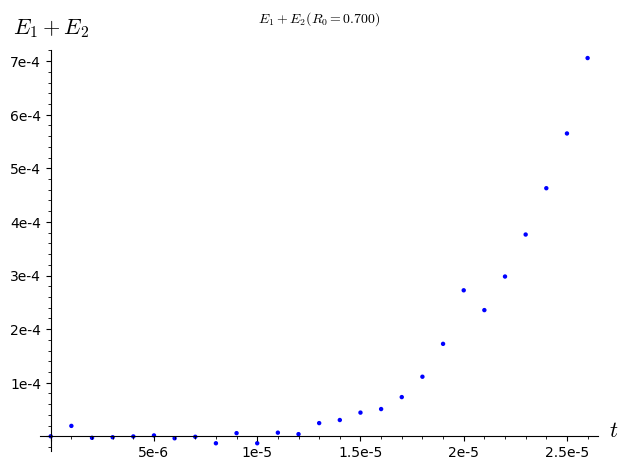
\includegraphics[scale=0.3]{spherical_explosion_E12_t_R0=0_700}
    \caption{Результат расчёта суммарного поля}
    \label{fig:spherical_explosion_E12_t_R0=0_700}
\end{wrapfigure}

Методом численного интегрирования с учетом запаздывания было вычислено результирующее электрическое поле в модели двойного электрического слоя со следующими параметрами: заряд обкладок 2.127 кулон,  начальный радиус 0.0002778 м (принятый как половина  ${R}_{1}$), ускорение положительной обкладки 2.778e6 $\frac{m}{sec^2}$ , ускорение отрицательной 9.489e8  $\frac{m}{sec^2}$, рассчитанные как ${a}_{R}$  для принятого начального радиуса. Начальная скорость обкладок нулевая.


\begin{wrapfigure}{r}{0.6\textwidth}
    \centering
    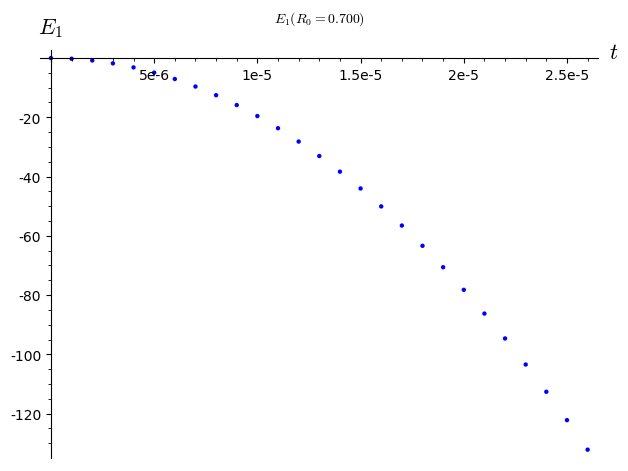
\includegraphics[scale=0.3]{spherical_explosion_E1_t_R0=0_700}
    \caption{Результат расчёта первой компоненты поля}
    \label{fig:spherical_explosion_E1_t_R0=0_700}
\end{wrapfigure}



Полученный результат показывает, что расчёт основанный на потенциалах Лиенара Вихерта не может показать отрицательную полярность импульса электрического поля, ускоряющегося двойного электрического слоя с внешней отрицательной обкладкой, который наблюдается в опыте.

\begin{wrapfigure}{l}{0.6\textwidth}
    \centering
    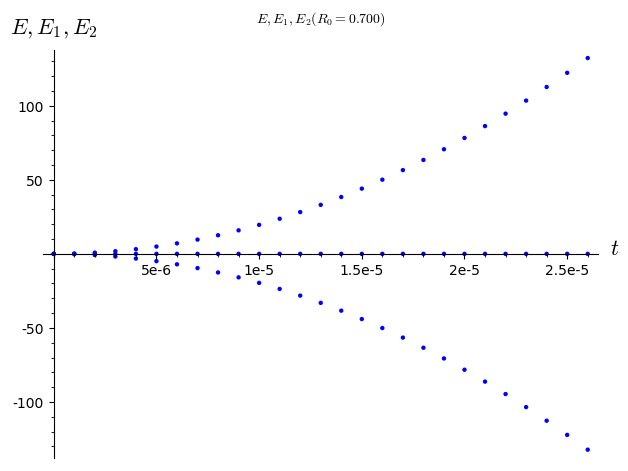
\includegraphics[scale=0.3]{spherical_explosion_E_E1_E2_t_R0=0_700}
    \caption{Результат расчёта первой второй компонент и их суммы}
    \label{fig:spherical_explosion_E_E1_E2_t_R0=0_700}
\end{wrapfigure}
%Чисто гипотетически отрицательную полярность импульса, ускоряющегося двойного электрического слоя, можно было бы получить, если изменить вторую компоненту электрического поля. Но как сделать так, чтобы это гипотетическое предположение соответствовало опыту? Ведь хорошо известно, что вторая компонента электрического поля получена обобщением результатов опытов по индукции Фарадея.


 
%Результат расчёта второй компоненты поля
 


 
%Оказывается, что если формулу для силы Лоренца разложить на сумму потенциальной и конвективной компонент, то можно показать, что, например, для случая движения контура в постоянном, но неоднородном магнитном поле, закон электромагнитной индукции Фарадея может быть объяснён как следствие действия только лишь конвективной компоненты силы Лоренца на электроны в проводнике контура.

%Следовательно, для того чтобы удовлетворить результатам опыта с ускоряющимся двойным электрическим слоем необходимо в формуле ${{E}_{2}}=-\frac{1}{c}\left( \frac{\partial }{\partial t}\overrightarrow{A} \right)$  ввести коэффициент зависящий от угла между направлением тока в источнике векторного потенциала $\overrightarrow{A}$ и направлением от источника векторного потенциала в точку наблюдения (в рамках данной работы этот угол уже введён как $\cos \left( \alpha  \right)'$  ), но для одновременного удовлетворения результатам опытов по электромагнитной индукции Фарадея достаточно сохранить знак и коэффициент только лишь для  $\cos \left( \alpha  \right)'=0$
 
 
%\[{{E}_{2}}=-\frac{k\left( \cos \left( \alpha  \right)' \right)}{c}\left( \frac{\partial }{\partial t}\overrightarrow{A} \right)\]
%\[k\left( \cos \left( \alpha  \right)'=0 \right)=1\] 
%\[k\left( \cos \left( \alpha  \right)'\ne 0 \right)<1\]


\section{О необходимости проведения контрольных опытов}

Поскольку результаты опыта Менде не удаётся объяснить исходя из уравнений классической электродинамики, то вполне ожидаемо появляются идеи связанные с усовершенствованием методики постановки эксперимента.

Идея 1. Если поменять полярность заряда конденсатора, изменится ли вид результирующих осциллограмм между внешним экраном и промежуточным экраном? Если при изменении полярности заряда конденсаторов вид результирующих осциллограмм изменится, тогда могут оказаться правы оппоненты, относящие данное явление на счёт классической Фарадеевой взаимоиндукции цепей разряда конденсаторов и цепей осциллографа.

Идея 2. Было бы полезно сравнить осциллограммы между внешним экраном и промежуточным экраном при наличии взрыва и при разряде конденсаторов через проволоку достаточно толстую настолько чтобы взрыва не было. При этом электрическое поле, возникающее непосредственно в результате взрыва, можно было бы оценить, как разность осциллограммы со взрывом и осциллограммы контрольного опыта без взрыва.

Предложенные здесь контрольные опыты, необходимы, чтобы удостовериться, что заявленный в публикации \cite{Mende2015} эффект действительно имеет место быть, и чтобы исключить возможность случайных помех или наводок на цепях осциллографа.

\section{Возможная связь с проблемой 4/3}

Проблема с неприменимостью потенциалов ЛВ к результатамопыта Менде со взрывом проволоки может иметь ту же природу, что и проблема 4/3.

Энрико Ферми в статье \cite{Fermi1923} 1923 года, 
%https://github.com/daju1/articles/blob/master/references/Stepanovsky/4_per_3/%D0%A4%D0%B5%D1%80%D0%BC%D0%B823.pdf
предлагает метод решения проблемы 4/3.

Применяя Гамильтонов метод с использованием аппарата теории относительности следующим образом: для вычисления действия нужно использовать переменные границы интегрирования для времени t1 и t2 Ферми приходит к соотношению (третья без номера формуле сверху на странице 80)

$$\int \vec E^{(i)} de + \int \vec E^{(i)}\frac{\vec a \vec R}{c^2} de + e \vec E^{(e)} + \int \vec E^{(e)}\frac{\vec a \vec R}{c^2} de = 0$$

Первое, он находит возможным пренебречь последним интегралом.

Второе. Он пишет, что $E^{(i)}$ это сумма сил Кулона и члена, содержащего ускорение. Действительно, чтобы получить для электромагнитной массы значение 4/3 нужно как например Батыгин и Топтыгин вычисляют инертную массу (в задаче 689 их задачника 1962 года издания), в качестве $E^{(i)}$ нужно взять поле по Лиенару Вихерту (при том что Батыгин и Топтыгин в этой задаче пренебрегают как запаздываение так и лоренцевым сокращением).

Если в качестве $E^{(i)}$ взять просто лишь кулоновское поле, как это сделал Ферми вычисляя интеграл в соотношении (4), то это только лишь потому что он пренебрёг слагаемыми интеграла которые содержат квадрат ускорения.

Давайте посмотрим насколько оправдано это пренебрежение.


В приближении малых скоростей ${}^{v} \big / {}_{c}\ll 1$  и малых ускорений $a{{r}_{0}}\ll {{c}^{2}}$ и при игнорировании запаздывания

Градиентное электрическое поле ($z$ компонента)
	\[{E}_{1}=\\
\int\limits_{{{r}_{q}}}\int\limits_{{{\varphi}_{q}}}\int\limits_{{{\theta}_{q}}}\\
\left\{ \frac{z_a-z_q}{{{R}_{0}}^3}\left( 1+\frac{a_z\left( {{z}_{a}}-{{z}_{q}} \right)}{c^2} \right) \\
 \right\}\\
{\rho \left( {{r}_{q}} \right){{r}_{q}}^{2}\sin \left( {{\theta }_{q}} \right)}\\
d{{\theta }_{q}}d{{\varphi }_{q}}d{{r}_{q}}\] 	

Электрическое поле самоиндукции ($z$ компонента)
\[{E}_{2}=\\
\int\limits_{{{r}_{q}}}\int\limits_{{{\varphi}_{q}}}\int\limits_{{{\theta}_{q}}}\\
{\left\{ -\frac{{a_z}}{{{c}^{2}}{{{R}_{0}}}} \right\}\\
{\rho \left( {{r}_{q}} \right){{r}_{q}}^{2}\sin \left( {{\theta }_{q}} \right)}\ }d{{\theta }_{q}}d{{\varphi }_{q}}d{{r}_{q}}\]
где ${R}_{0}$ расстояние от точки источника заряда к точке наблюдения без учёта запаздывания.

Записывая в обозначениях близких к работе Ферми, обозначая как ${E}^{(i)}$ поле, обусловленное самой системой

\[{E}^{(i)}={E}_{1}+{E}_{2}=\\
\int\left\{ \frac{z_a-z_q}{{{R}_{0}}^3}+\frac{a_z\left( {{z}_{a}}-{{z}_{q}} \right)^2}{c^2{{{R}_{0}}^3}} - \frac{{a_z}}{{{c}^{2}}{{{R}_{0}}}}\\
\right\}\\de'\]

Вычисляя инертную массу электрона с помощью потенциалов ЛВ, получаем вслед за Батыгиным-Топтыгиным 4/3
%https://github.com/daju1/articles/blob/master/sagemath/inertial_mass_of_charged_particle/About_inertial_properties_of_electromagnetic_mass.01.pdf


\[\int {E}^{(i)} de = \int\int \left\{ \frac{z_a-z_q}{{{R}_{0}}^3}+\frac{a_z\left( {{z}_{a}}-{{z}_{q}} \right)^2}{c^2{{{R}_{0}}^3}}  -\frac{{a_z}}{{{c}^{2}}{{{R}_{0}}}}
 \right\}\\
de de'\]

для равномерно по всему объёму заряженной сферы

\[\int {E}^{(i)} de = \left\{ 0 - \frac{2}{5}  - \frac{6}{5} \right\}\frac{a_z e^2}{ c^2{{{R}}}}\\
\]	

Учитывая что для равномерно заряженной по всему объему сферы

\[u = \frac{3}{5}\frac{e^2}{R}\]

находим

\[\int {E}^{(i)} de = -\frac{4}{3} \cdot 2\frac{u}{c^2}\,a_z.\\
\]	

 Соотношение (4) из работы Ферми, если записать его в современных обозначениях будет выглядеть так:

$$-\frac{4}{3}\cdot 2 \,\frac{u}{c^2} \, a_z + \int \vec E^{(i)}\frac{\vec a \vec R}{c^2} de + \vec F = 0$$

Подставляя выражение для ${E}^{(i)}$


$$-\frac{4}{3}\cdot 2 \,\frac{u}{c^2} \, a_z + \int \int
\left\{ \frac{z_a-z_q}{{{R}_{0}}^3}+\frac{a_z\left( {{z}_{a}}-{{z}_{q}} \right)^2}{c^2{{{R}_{0}}^3}}  -\frac{{a_z}}{{{c}^{2}}{{{R}_{0}}}}\\
 \right\}\\
de'\frac{\vec a \vec R}{c^2} de + \vec F = 0$$

и учитывая, что ускорение имеет только лишь $z$ компоненту

$$-\frac{4}{3}\cdot 2 \,\frac{u}{c^2} \, a_z + \int \int
\left\{ \frac{z_a-z_q}{{{R}_{0}}^3}+\frac{a_z\left( {{z}_{a}}-{{z}_{q}} \right)^2}{c^2{{{R}_{0}}^3}}  -\frac{{a_z}}{{{c}^{2}}{{{R}_{0}}}}\\
 \right\}\\
de'\frac{a_z \left(z_a-z_q\right)}{c^2} de + \vec F = 0$$


$$-\frac{4}{3}\cdot 2 \,\frac{u}{c^2} \, a_z + \int \int
\left\{ \frac{a_z\left(z_a-z_q\right)^2}{{c}^{2}{{R}_{0}}^3}+\frac{a_z^2\left( {{z}_{a}}-{{z}_{q}} \right)^3}{c^4{{{R}_{0}}^3}}  -\frac{{a_z^2}\left(z_a-z_q\right)}{{{c}^{4}}{{{R}_{0}}}}\\
 \right\}\\
de' de + \vec F = 0$$

Учитывая численное значение первого интеграла для равномерно заряженной по объёму сферы

$$-\frac{4}{3}\cdot 2 \,\frac{u}{c^2} \, a_z + \frac{2}{5} \frac{a_z e^2}{c^2{R}} + \int \int \left\{
\frac{a_z^2\left( {{z}_{a}}-{{z}_{q}} \right)^3}{c^4{{{R}_{0}}^3}}  -\frac{{a_z^2}\left(z_a-z_q\right)}{{{c}^{4}}{{{R}_{0}}}}\\
 \right\}\\
de' de + \vec F = 0$$

И подставляя значение электростатической энергии

$$-\frac{4}{3}\cdot 2 \,\frac{u}{c^2} \, a_z + \frac{1}{3} \cdot 2 \, \frac{u}{c^2} a_z + \int \int \left\{
\frac{a_z^2\left( {{z}_{a}}-{{z}_{q}} \right)^3}{c^4{{{R}_{0}}^3}}  -\frac{{a_z^2}\left(z_a-z_q\right)}{{{c}^{4}}{{{R}_{0}}}}\\
 \right\}\\
de' de + \vec F = 0$$


Приходим к выражению 

$$\vec F =  2 \,\frac{u}{c^2} \, a_z - \int \int \left\{
\frac{a_z^2\left( {{z}_{a}}-{{z}_{q}} \right)^3}{c^4{{{R}_{0}}^3}}  -\frac{{a_z^2}\left(z_a-z_q\right)}{{{c}^{4}}{{{R}_{0}}}}\\
 \right\} de' de.$$

В этом выражении множитель 2 перед ${u}/{c^2}$ соответствует определению классического радиуса электрона из Википедии, который \begin{itshape}"равен радиусу заряженной сферы (на которой равномерно распределён заряд), если этот заряд равен заряду электрона, а потенциальная энергия электростатического поля $\textbf{u}$ полностью эквивалентна \textbf{половине} массы электрона"\end{itshape}.

% И третье. Он берет полусумму и не объясняет почему. А полусумма берется при вычислении энергии кулоновского поля. А вот при вычислении силы самодействия полусумма не берется на мой взгляд, потому что нужно учесть как силу самодействия на de так и на de'. При вычислении силы самодействия берётся именно сумма а не полусумма.


Ферми показал дополнительный интеграл (равный -1/3), имеющий отрицательный знак, который нужно использовать чтобы решить проблему 4/3.

Исходя из формализма ЛВ этот дополнительный интеграл Ферми как раз равен половине градиентного интеграла который возникает при решении задачи об инертной массе электрона методом ЛВ. А градиентный интеграл это интеграл поля $E_1$ в обозначениях текущей работы. Знак компоненты поля $E_1$, полученный в данной работе, отрицательный. Если увеличить, вслед за Ферми, величину градиентного интеграла $E_1$ (Ферми его увеличил в полтора раза), то можно получить отрицательный знак электрического импульса центрально симметричного взрыва плазмы, как это показано в публикации Менде.

И таким образом все сходится. По крайней мере получается качественное сходство теории и практики.

Но теперь возникает вопрос: как на практике для точного решения практических задач использовать потенциалы Лиенара Вихерта с учётом ${}^{4}/{}_{3}$ поправки Энрико Ферми?

% Каждый раз вводить поправку увеличивая градиентную компоненту поля? Тогда как эта поправка должна выглядеть....

Суммарное электрическое поле по Лиенару Вихерту

$$\vec{E} = \frac{dq}{{{R}^{*}}^{3}}\left( \left(\vec{R}-\frac{R}{c}\vec{v} \right) \left(1 + \frac{\vec{R}\vec{a}}{c^2} - \frac{v^2}{c^2} \right) - \vec{a}\,\frac{{R}^{*}R}{c^2} \right)$$

получено в электродинамике (см. например ЛЛ2, $"$Теория поля$"$, параграф 63, формула (63,8)) исходя из вариации действия типа А, противоречащей принципу относительности. Но для того, чтобы получить поле, соответствующее вариации типа В, необходимо поле Лиенара Вихерта дополнить множителем Ферми $\left(1 + \frac{\vec{R}\vec{a}}{c^2}\right)$, возникшим благодаря искривлению мировой трубки в 4-пространстве при движении заряда с ускорением.

Таким образом, новая формула поля, назовём ее поле Лиенара-Вихерта-Ферми, имеет вид:

$$\vec{E} = \frac{dq}{{{R}^{*}}^{3}}\left( \left(\vec{R}-\frac{R}{c}\vec{v} \right) \left(1 + \frac{\vec{R}\vec{a}}{c^2} - \frac{v^2}{c^2} \right) - \vec{a}\,\frac{{R}^{*}R}{c^2} \right) \left(1 + \frac{\vec{R}\vec{a}}{c^2}\right).$$


\begin{thebibliography}{99}

\bibitem{Apfelbaum2009}
\textit{Apfelbaum, E. a. (2009). The predictions of the critical point parameters for Al, Cu and W found from the correspondence between the critical point and unit compressibility line (Zeno line) positions. Chemical Physics Letters(467), pp. 318–322. Retrieved from https://www.sciencedirect.com/science/article/abs/pii/S0009261408015790}

\bibitem{Baker1964}
\textit{Baker, D. A. (1964). Second-Order Electric Field due to a Conducting Curent. American Journal of Physics, 32(2), 153-157.}

\bibitem{Edwards1976}
\textit{Edwards, W. F. (1976). Continuing investigation into possible electric arising from steady conduction current. Phys. Rev. D, 14(4), 922--938. doi:10.1103/PhysRevD.14.922}

\bibitem{Mende1993}
\textit{Mende, F. F. (1993). Conference “Physics in Ukraine”. Experimental corroboration and theoretical interpretation of dependence of charge value on DC flow velocity through superconductors. Kiev.
Roser, W. (1962). Second-Order Electric Field due to a Conducting Curent. American Journal of Physics, 30(7), 509-511.}

\bibitem{Roser1962}
\textit{Roser, W. (1962). Second-Order Electric Field due to a Conducting Curent. American Journal of Physics, 30(7), 509-511.}

\bibitem{rustot}
\textit{Re: Как запаздывающий Лиенар-Вихерт становится "незапаздывающим". Визуализация}
\\\texttt{http://www.sciteclibrary.ru/cgi-bin/yabb2/YaBB.pl?num=1528093569/330\#330}

%\textit{rustot5. (б.д.). Re: Как запаздывающий Лиенар-Вихерт становится "незапаздывающим". Визуализация. Получено из Научно-технический форум SciTecLibrary: http://www.sciteclibrary.ru/cgi-bin/yabb2/YaBB.pl?num=1528093569/326\#326}

%http://www.sciteclibrary.ru/cgi-bin/yabb2/YaBB.pl?num=1528093569/415\#415

\bibitem{Adamyan1999}
\textit{Адамьян Ю.Э., В. В. (1999). Нагрев и ускорение плазмы при взрыве проводника в вакууме в сильном магнитном поле. Журнал технической физики, 69(5).}

\bibitem{Dobrovolskaya2015}
\textit{Добровольская А.С., К. Н. (2015). Применение дискретной кинетической модели для системы уравнений Эйлера - Пуассона к задачам плазменной аэродинамики. Физико-химическая кинетика в газовой динамике, 16(3). Получено из http://chemphys.edu.ru/issues/2015-16-3/articles/571/}

\bibitem{Zinovyev1989}
\textit{Зиновьев, В. (1989). Теплофизические свойства металлов при высоких температурах. «Металлургия».}

\bibitem{Mende2013}
\textit{Менде, Ф. Ф. (2013). Электрический импульс космического термоядерного взрыва. Инженерная физика, 16-24.}

\bibitem{Mende2015}
\textit{Менде, Ф. Ф. (2015). Является ли заряд инвариантом скорости?}% Получено из % http://fmnauka.narod.ru/javljaetsja_li_zarjad_invariantom_skorosti.pdf

\bibitem{Sasakin2016}
\textit{Сасакин, М. (2016). Разлёт в вакуум и взаимодействие с преградой мелкодисперсных частиц при электрическом взрыве проводника. Санкт-Петербург.}

\bibitem{Tamm1957}
\textit{Тамм, И. (1957). Основы теории электричества. Москва.}

\bibitem{Chirkin1968}
\textit{Чиркин, В. (1968). Теплофизические свойства материалов ядерной техники. Справочник. М: Атомиздат.}

\bibitem{Fermi1923}
\textit{Ферми, Энрико. (1923). Разрешение существующего противоречия между электродинамической и релятивистской теориями электромагнитной массы. Энрико Ферми, т.1 стр. 73}



\end{thebibliography}

\end{document}



